\begin{frame}
    \frametitle{Graph-SLAM}
    
    Graph-SLAM: Construct a graph and find a configuration of nodes that minimizes the error introduced by constraints (edges)
    
    \begin{itemize}
    \item A graph is used to represent the problem.
    \item The nodes represent poses or locations of landmarks.
    \item Edges are landmark observations or odometry measurements
    \item Minimization optimizes robot poses and landmark placement
    \item Observing previously viewed areas generates constraints in the graph
    \end{itemize}
    
    \begin{figure}
    \subfloat[]
    {
    \fbox{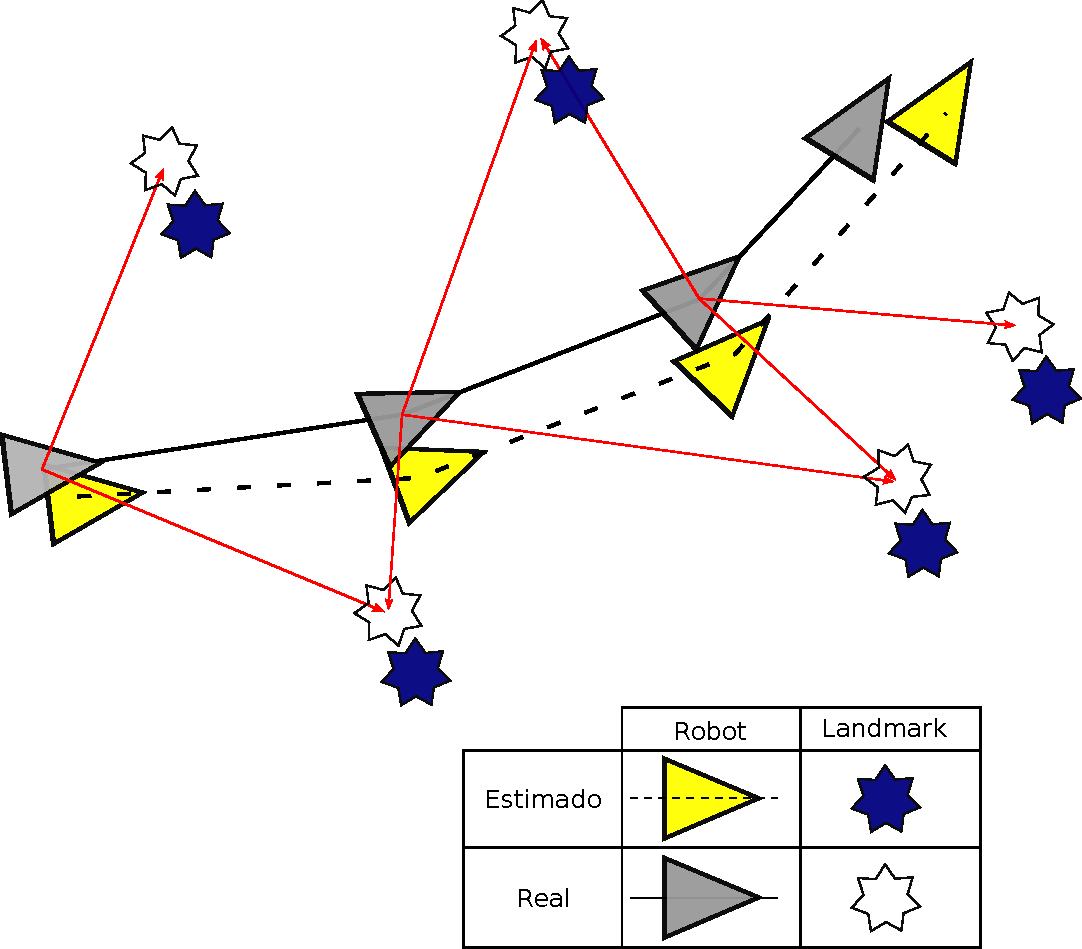
\includegraphics[width=0.25\textwidth]{images/slam-landmarks.pdf}}
    }\hspace{1em}
    \subfloat[]
    {
    \fbox{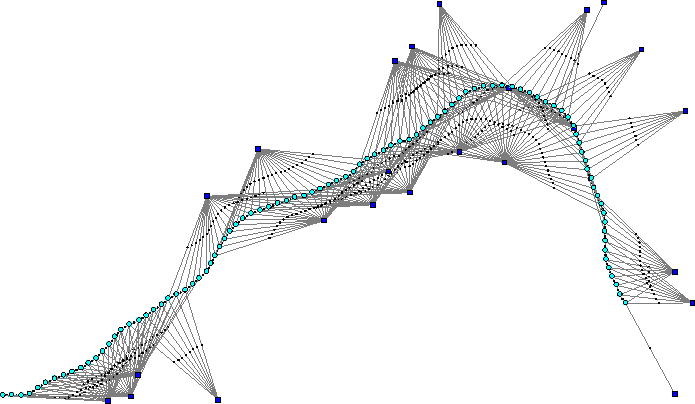
\includegraphics[width=0.375\textwidth]{images/factor_graph.pdf}}
    }
    \end{figure}
    
    \end{frame}
    
    \begin{frame}
    \frametitle{Factor-Graph}
    \note{Information taken from https://youtu.be/uuiaqGLFYa4}
    
    \begin{block}{Factor-Graph}
    A Factor-graph is a mathematical term, a bipartite graph (Nodes: Variables and Factors and Edges: determine the variables on which the factors depend) representing the factorization of a function. This means that we can take a function, for example, $g(.)$ and decompose it by the product of functions $f(.)$,
    
    \begin{equation*}
    g(X_{1}, \dots, X_{n}) = \prod_{i} f_{i}(S_{i}) \quad \text{con} \quad S_{i} \subseteq \{ X_{1},\dots, X_{n} \}
    \end{equation*}
    \end{block}
    
    \begin{figure}[!h]
    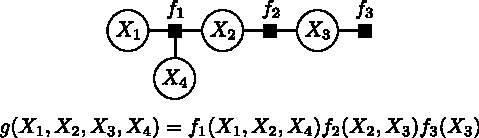
\includegraphics[width=0.7\textwidth]{images/factor_graph_example.pdf}
    \end{figure}
    
    \note{For example, if the function g depends on 10 variables, we can decompose it into the product of several functions f, where each function f depends on a subset of those variables.}
    
    \end{frame}
    
    \begin{frame}
    \frametitle{Factor-Graph}
    \note{Information taken from https://youtu.be/uuiaqGLFYa4}
    
    \begin{itemize}
    \item Factor-graphs allow us to represent a joint probability distribution (a distribution that governs all variables) as a product of smaller probabilities (which depend on a smaller number of variables).
    \item Like Bayes networks or Markov networks, we can use Factor-graphs to describe how variables depend on each other. And we can run different algorithms on these Factor-graphs to efficiently infer information.
    \item An example of an algorithm that works on a Factor-graph is the Sum-Product Algorithm for computing marginal distributions (distributions that only depend on a subset of variables).
    \item In the context of robotics, Factor-graphs are used to specify least squares problems. The factor graph allows us to represent how certain states depend on or are related to each other based on the information we have from sensor measurements (stored in the factors).
    \end{itemize}
    
    \note{For example, if function g depends on 10 variables, we can decompose it into the product of several functions f, where each function f depends on a subset of those variables.}
    
    \end{frame}
    
    \begin{frame}
    \frametitle{Graph-based SLAM using Pose-Graph}
    \note{Information taken from https://youtu.be/uHbRKvD8TWg}
    
    \begin{itemize}
    \item The constraints connect the robot's poses as it moves.
    \item The constraints are noisy.
    \end{itemize}
    
    \begin{figure}[!h]
    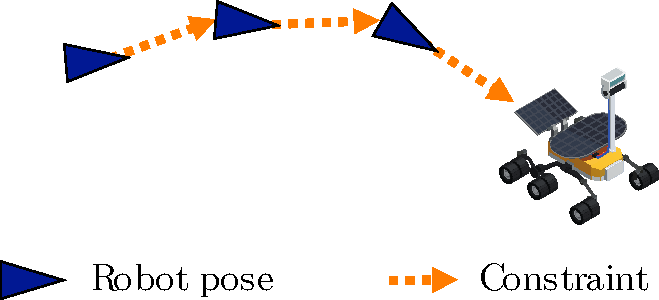
\includegraphics[width=0.7\textwidth]{images/pose_graph_example.pdf}
    \end{figure}
    
\end{frame}

\begin{frame}
    \frametitle{Graph-based SLAM using Pose-Graph}
    \note{Information taken from https://youtu.be/uHbRKvD8TWg}
   
    \begin{itemize}
    \item By observing previously seen areas, restrictions are generated between non-consecutive poses (\emph{Loop Closure})
    \end{itemize}
   
    \begin{figure}[!h]
    \includegraphics[width=0.4\textwidth]{images/pose_graph_loop_example.pdf}
    \end{figure}
   
   \end{frame}
   
   \begin{frame}[fragile]
    \frametitle{2D Pose-Graph with LiDAR}
    \note{Video taken from https://youtu.be/E6IvbjZA7Ao}
   
    \begin{center}
   \movie[loop]{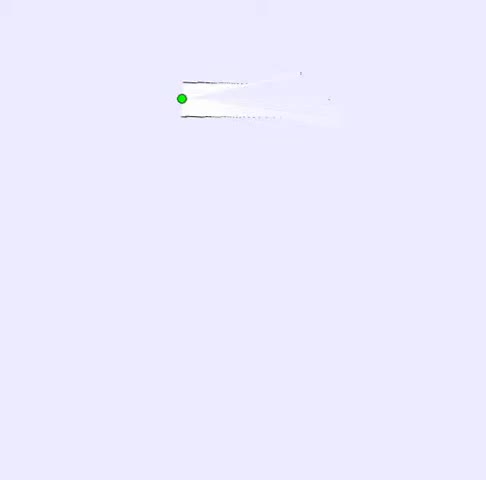
\includegraphics[width=0.5\columnwidth]{./images/pose_graph_2d_video.jpg}}{./videos/pose_graph_2d.mp4}
   \end{center}
   
   \end{frame}
   
   \begin{frame}
   \frametitle{Graph-based SLAM using Pose-Graph}
   \note{Information taken from https://youtu.be/uHbRKvD8TWg}
   
   \begin{columns}
   \begin{column}{0.5\textwidth}
   \begin{itemize}
   \item<1-2> Each node is a robot pose along with its laser measurement (there are no landmarks)
   \item<1-2> Each edge corresponds to a spatial constraint between the nodes it relates. \item<3-> Once we have the graph, we obtain the most probable map by correcting the nodes
    \item<4-> like this...
    \item<5> We draw the map based on the corrected poses
    \end{itemize}
    \end{column}
    \begin{column}{0.5\textwidth} %%<--- here
    \only<1>{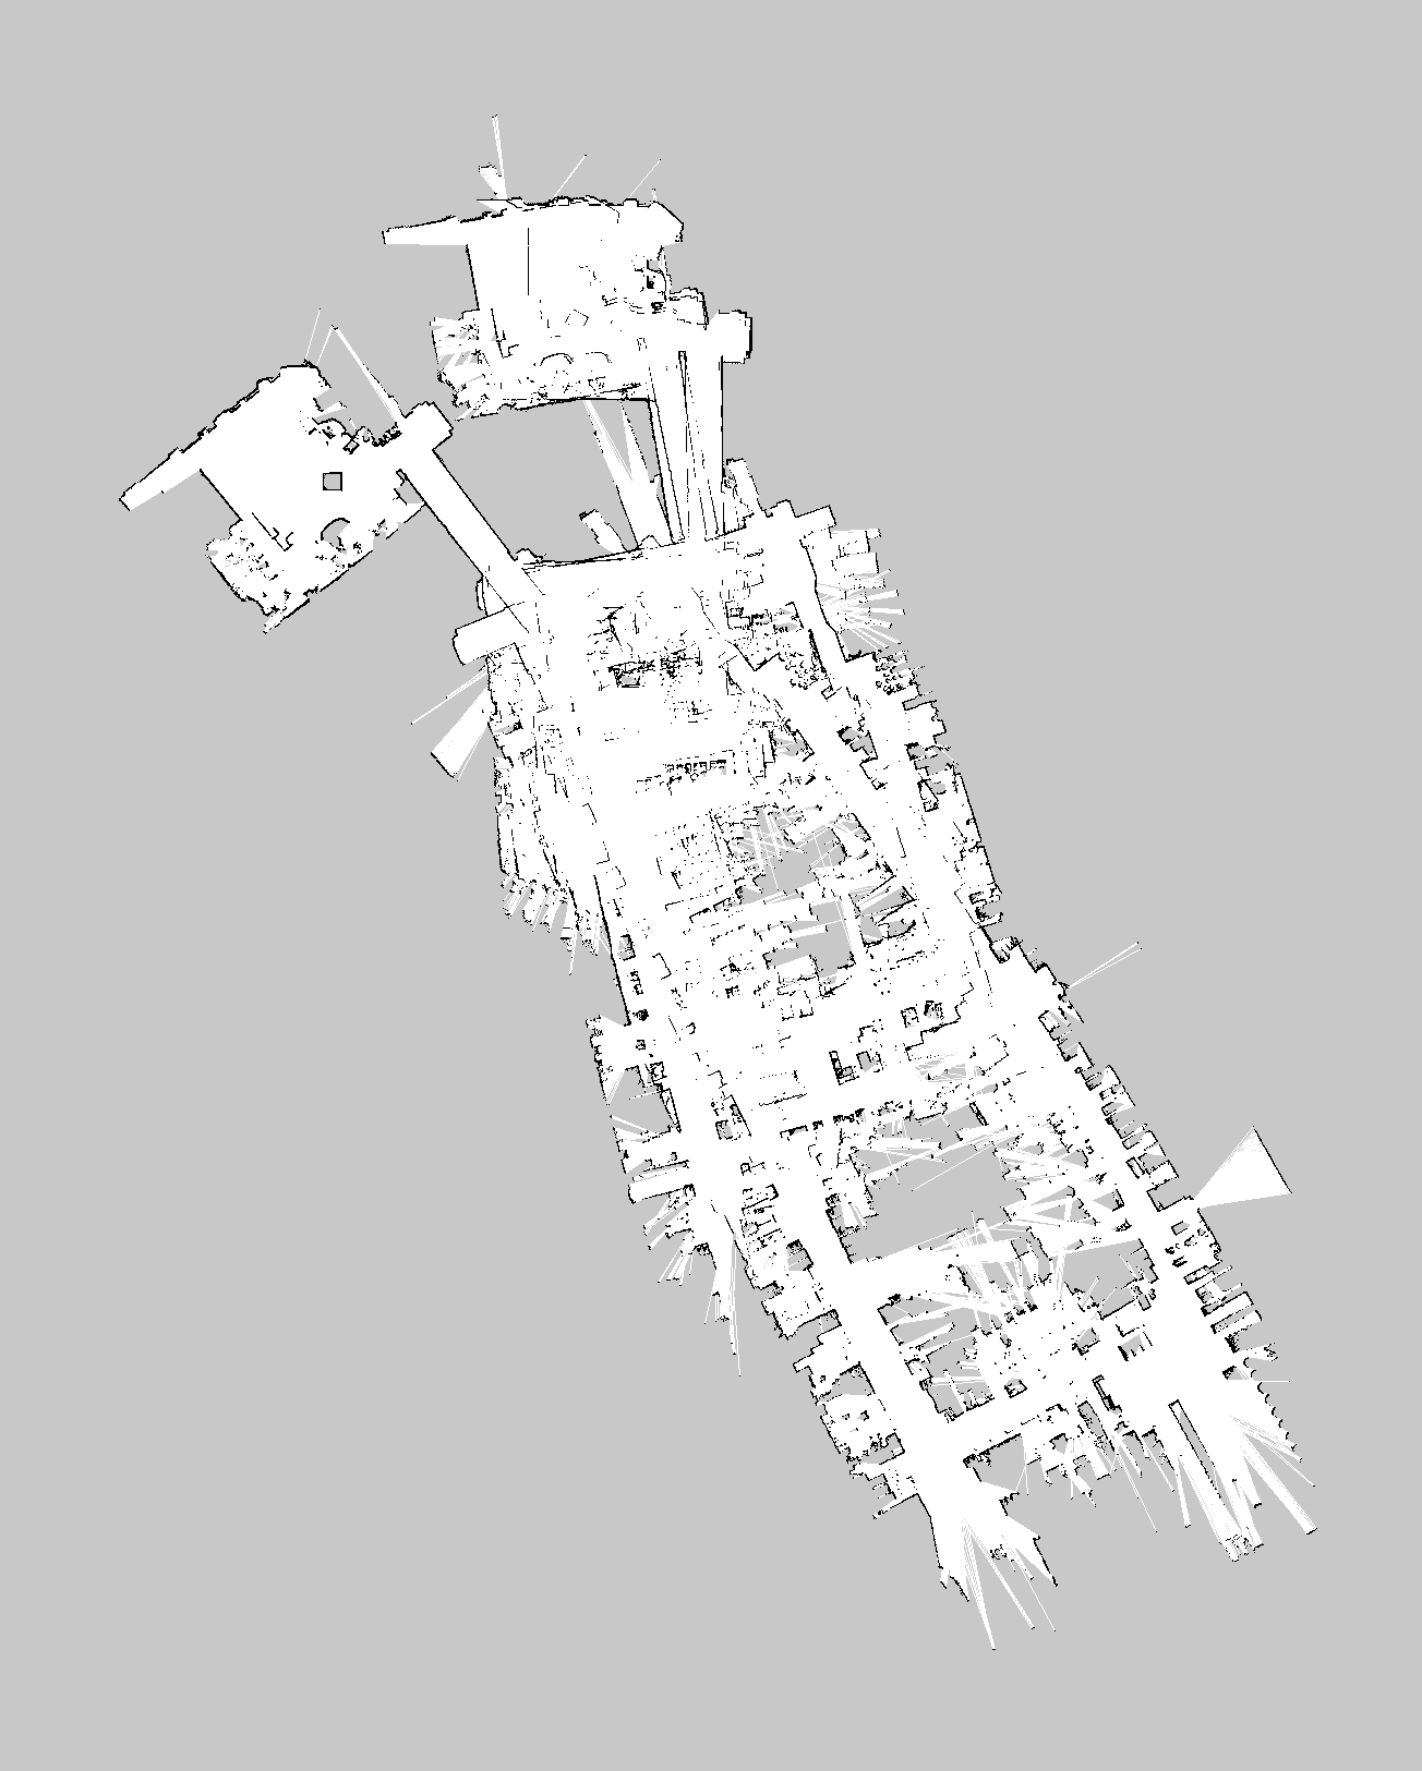
\includegraphics[width=0.7\textwidth]{images/pose_graph_map.png}}
    \only<2>{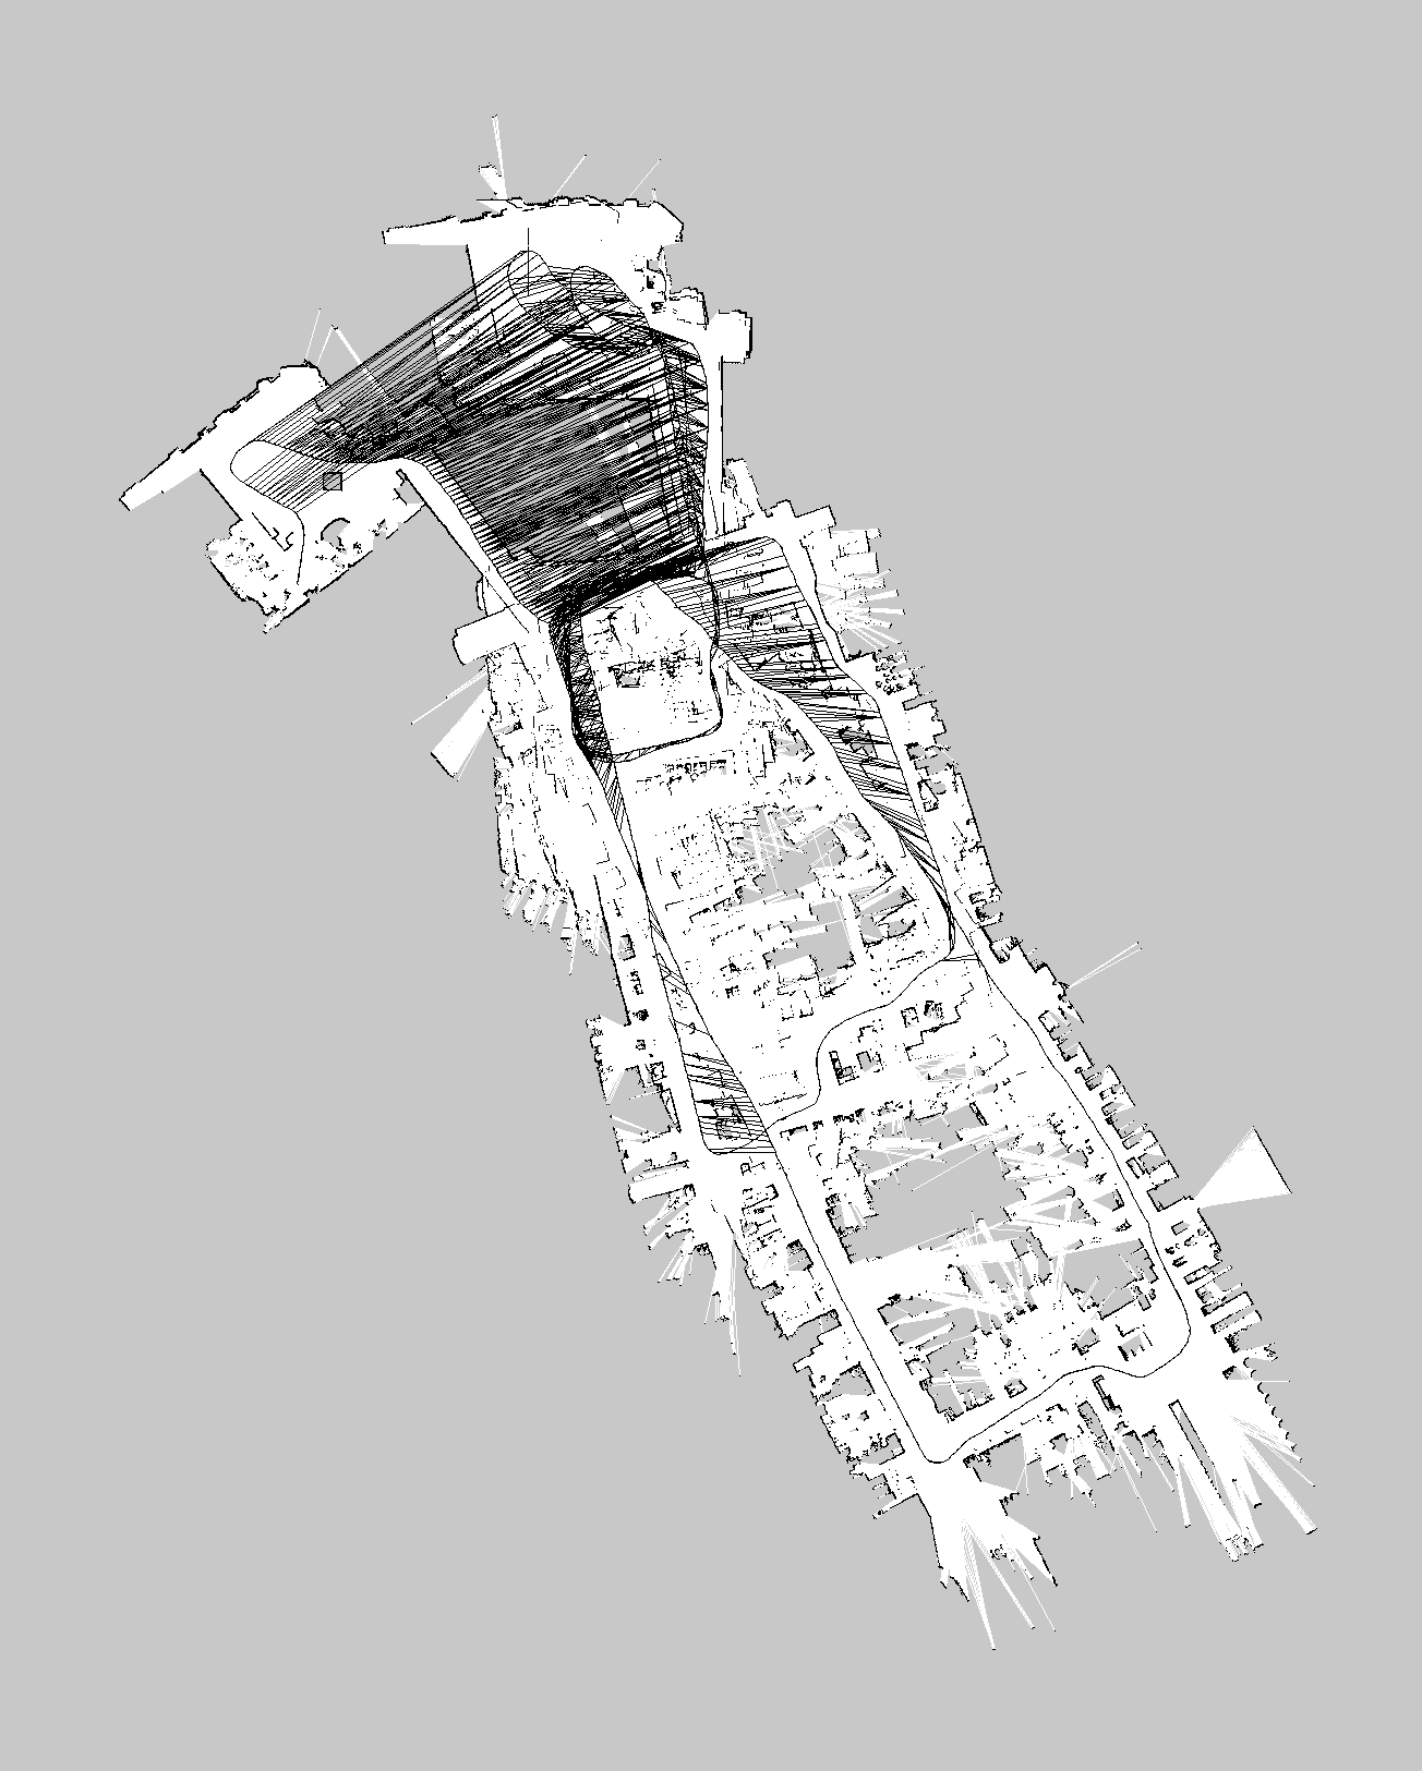
\includegraphics[width=0.7\textwidth]{images/pose_graph_constraints_with_map.png}}
    \only<3>{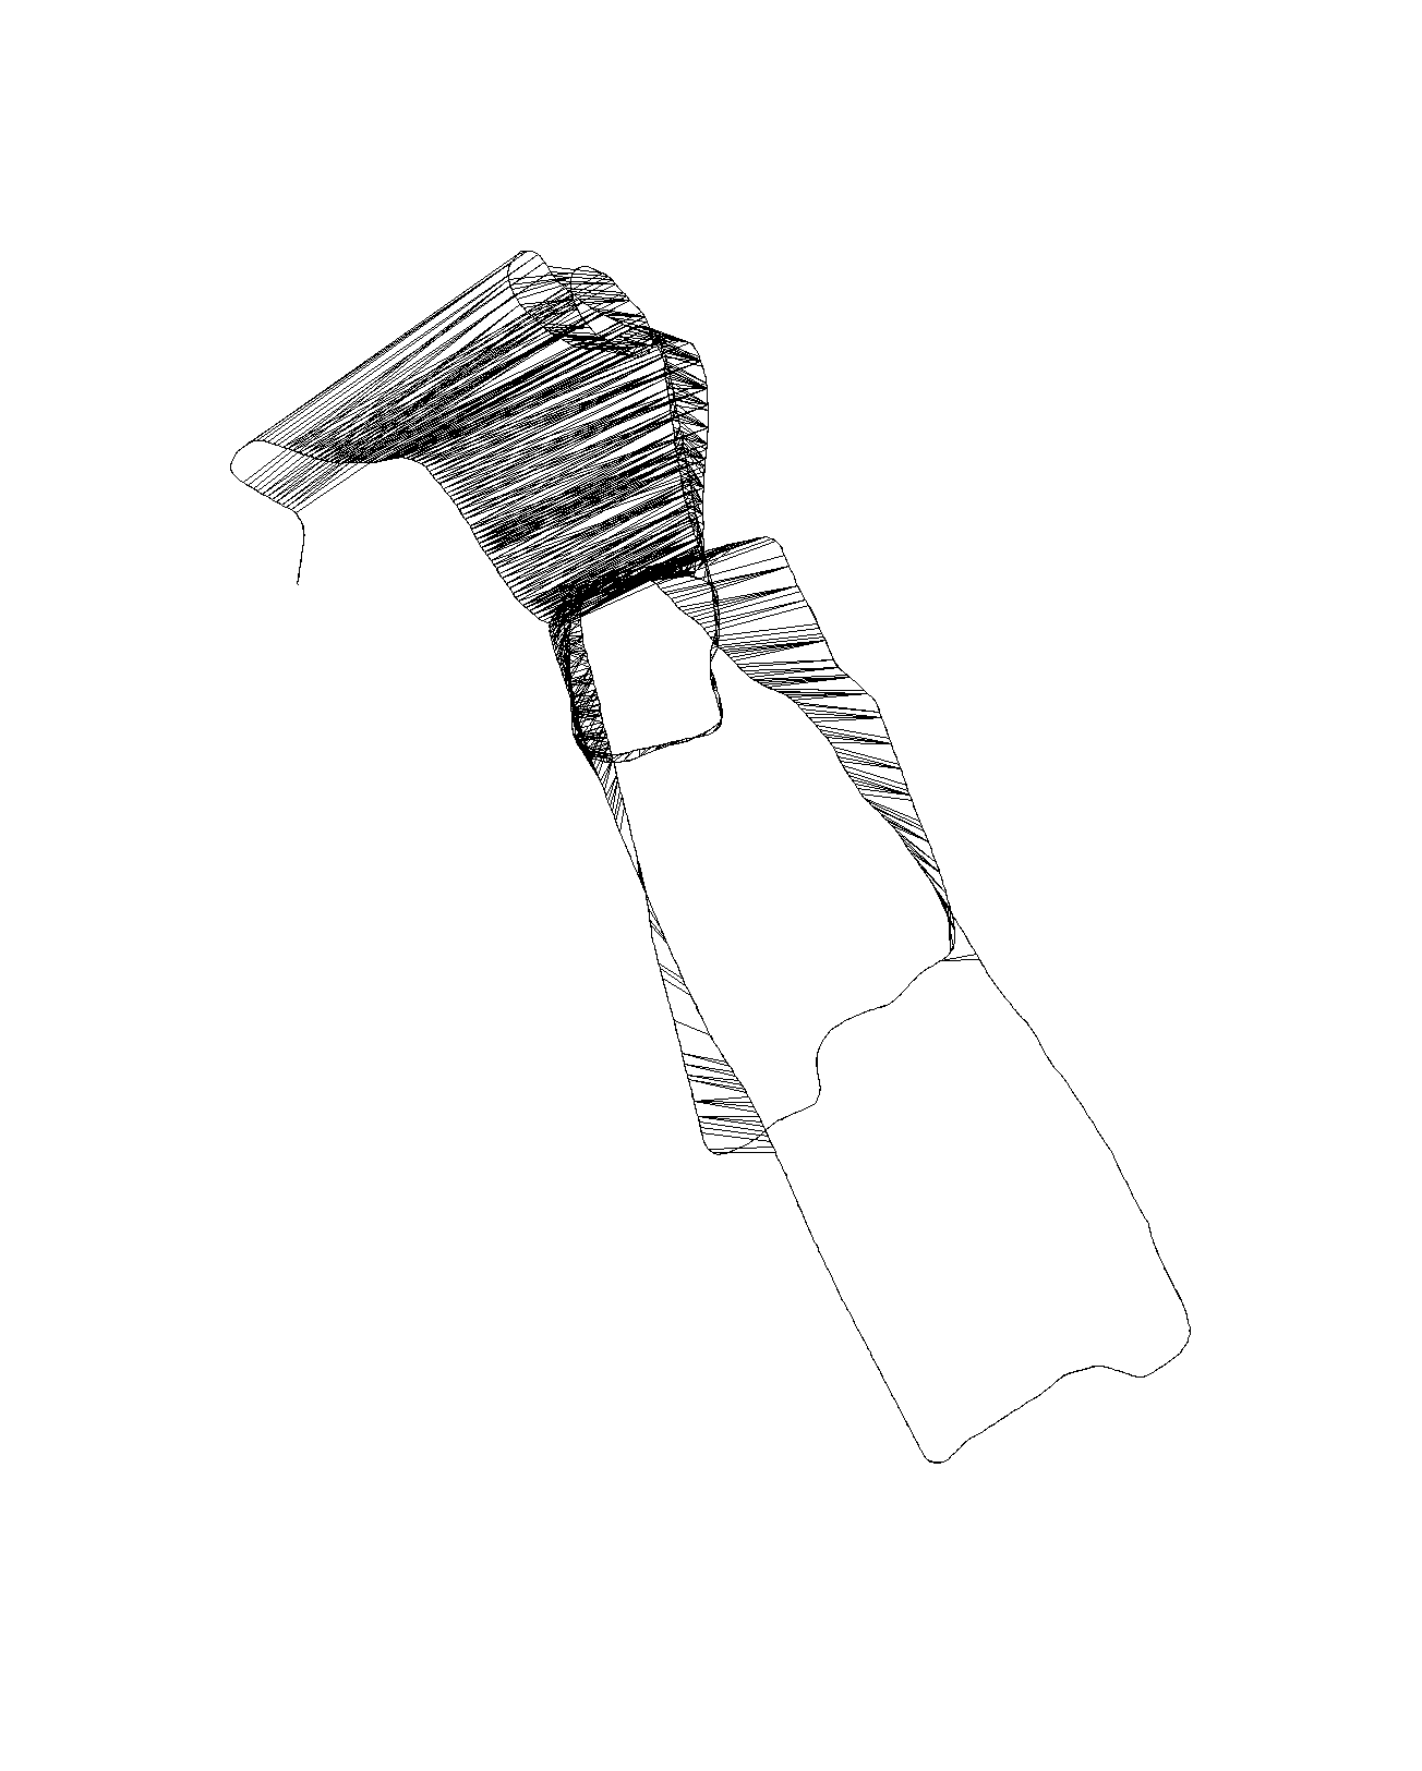
\includegraphics[width=0.7\textwidth]{images/pose_graph_constraints.png}}
    \only<4>{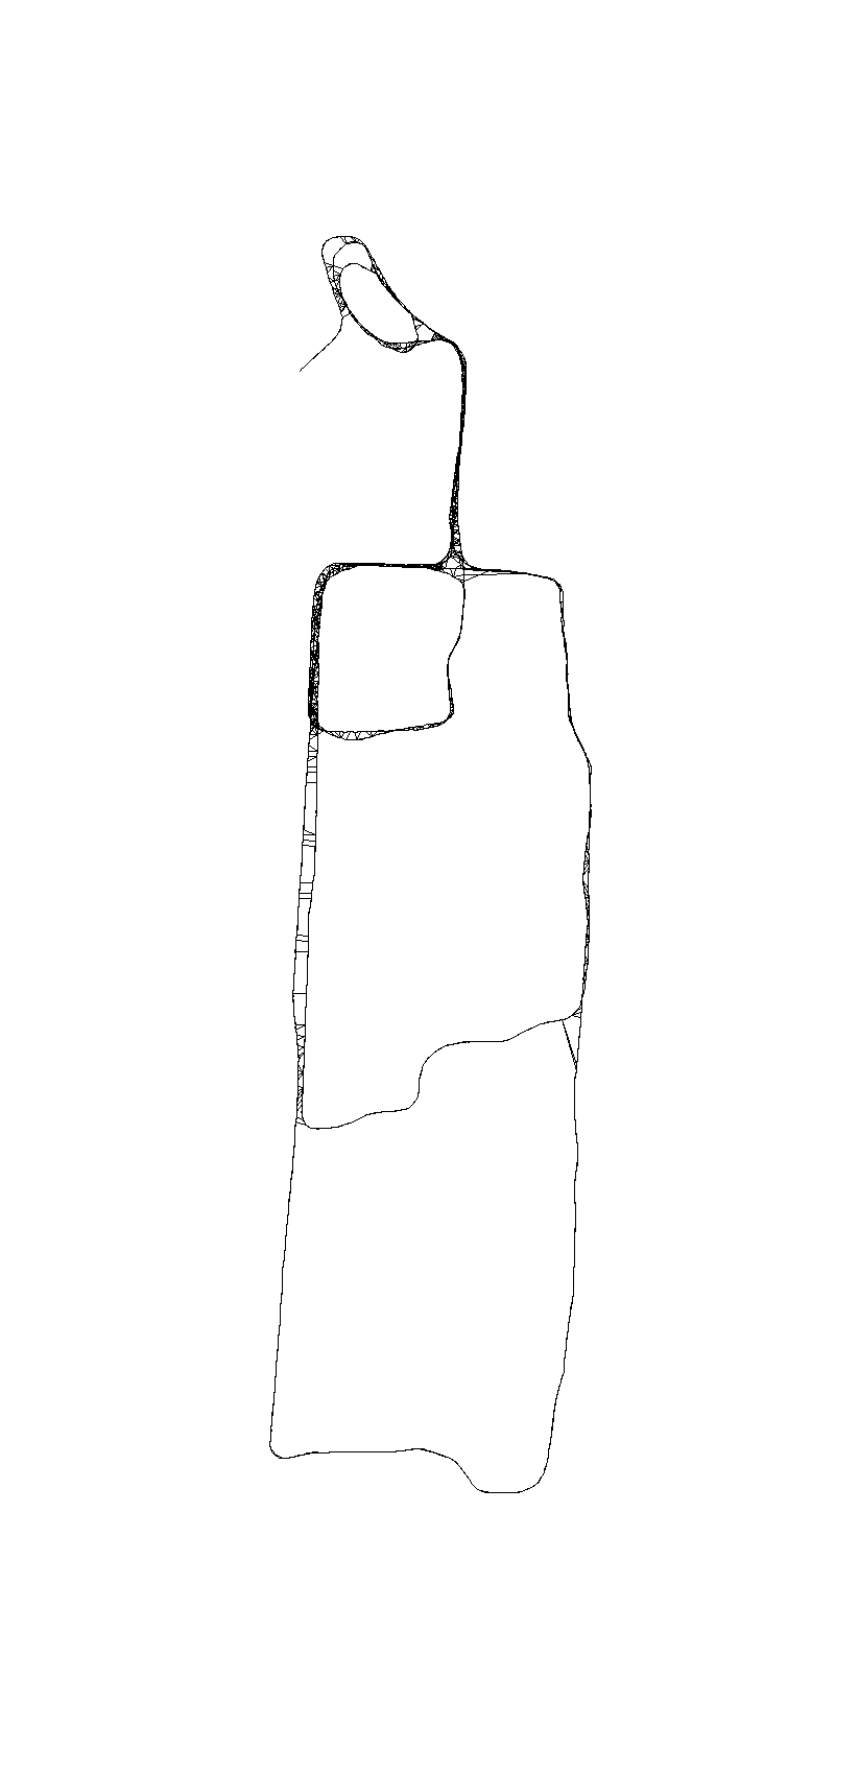
\includegraphics[width=0.5\textwidth]{images/pose_graph_optimized.png}}
    \only<5>{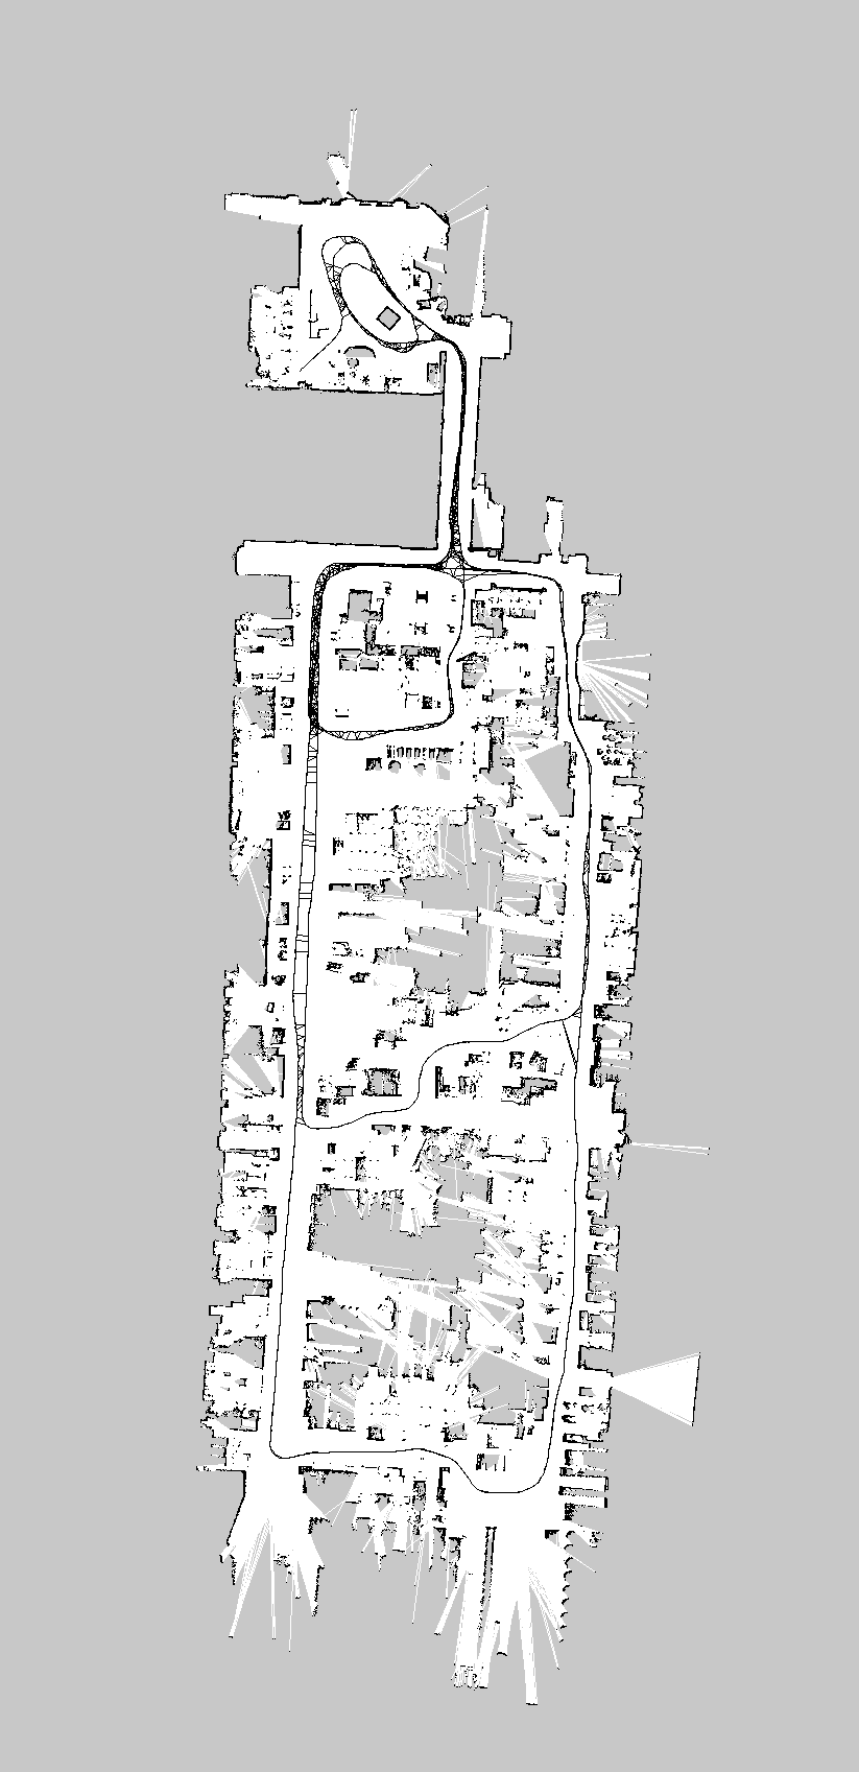
\includegraphics[width=0.5\textwidth]{images/pose_graph_optimized_with_map.png}}
    \end{column}
    \end{columns}
   
   \end{frame}
   
   \begin{frame}
    \frametitle{The graph in pose-graph}
    \note{Information taken from https://youtu.be/uHbRKvD8TWg}
   
    \begin{itemize}
    \item Consists of $n$ nodes $\stateBold = \stateBold_{1:n}$
    \item Each $\stateBold_{i}$ is a pose of the robot at time $t_{i}$
    \item A constraint/edge exists between node $\stateBold_{i}$ and $\stateBold_{j}$ if...
   \end{itemize}
   
   \begin{figure}[!h]
   \includegraphics[width=0.3\textwidth]{pose_graph_loop_example.pdf}
   \end{figure}
   
   \end{frame}
   
   \begin{frame}
   \frametitle{Create an edge if...}
   \note{Information taken from https://youtu.be/uHbRKvD8TWg}
   
   \begin{itemize}
   \item A constraint/edge exists between node $\stateBold_{i}$ and $\stateBold_{j}$ if the robot moves from $\stateBold_{i}$ to $\stateBold_{i+1}$
   \item The edges correspond to odometry
   \end{itemize}
   
   \begin{figure}[!h]
   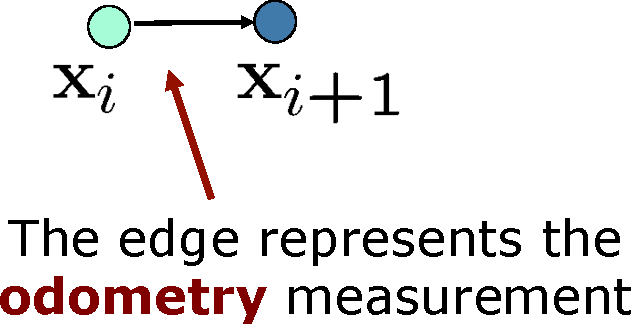
\includegraphics[width=0.44\textwidth]{pose_graph_odometry_edge.pdf}
   \end{figure}
   
   \end{frame}
   
   \begin{frame}
   \frametitle{Create an edge if...}
   \note{Information taken from https://youtu.be/uHbRKvD8TWg}
   
   \begin{itemize}
   \item<1-> A constraint/edge exists between node $\stateBold_{i}$ and $\stateBold_{j}$ if the robot observes the same part of the environment from $\stateBold_{i}$ and from $\stateBold_{j}$
   \item<2> We construct a {\bf virtual constraint} between the position of $\stateBold_{j}$ as seen from $\stateBold_{i}$
   \end{itemize}
   \only<1>{
   \begin{figure}
   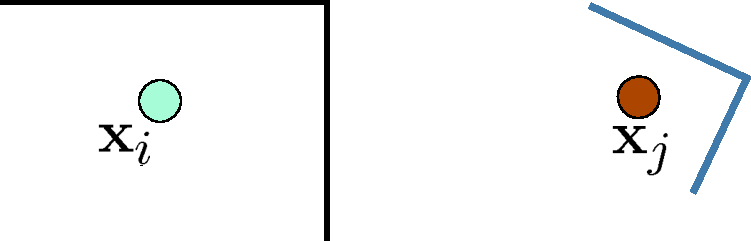
\includegraphics[width=0.44\textwidth]{pose_graph_edge_lidar.pdf}
   \end{figure}
   }
   \only<2>{
   \begin{figure}
   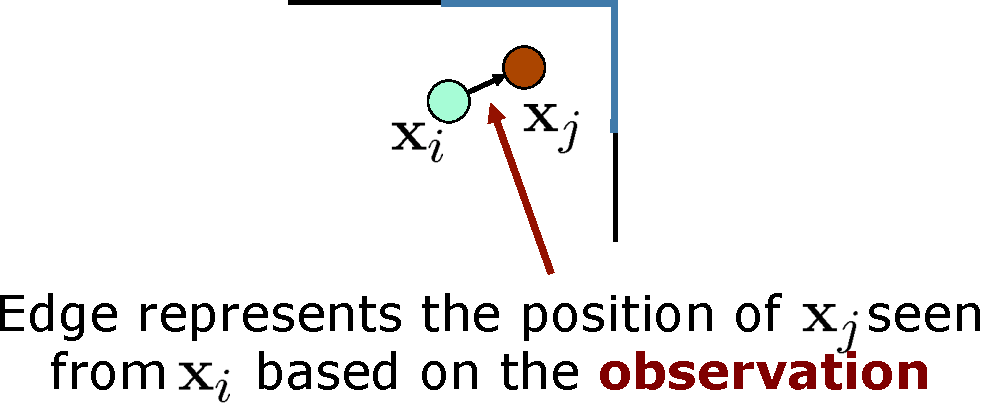
\includegraphics[width=0.44\textwidth]{pose_graph_edge_lidar2.pdf}
   \end{figure}
   }
   
   \end{frame}
   
   \begin{frame}
   \frametitle{The edge information matrix}
   \note{Information taken from https://youtu.be/uHbRKvD8TWg}
   \begin{itemize}
   \item Observations are noisy
   \item The information matrix $\informationMatrix_{ij}$ for each edge encodes its uncertainty
   \item The larger the $\informationMatrix_{ij}$, the more important the edge is in the optimization.
   \end{itemize}
   
   \end{frame}
   
   \begin{frame}
    \frametitle{The edge information matrix}
    \note{Information taken from https://youtu.be/uHbRKvD8TWg}
    \begin{figure}[!h]
    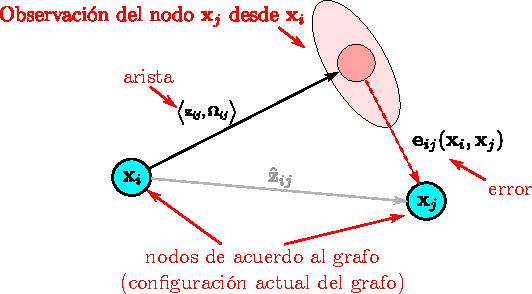
\includegraphics[width=0.7\textwidth]{images/factor_graph_edge_example.pdf}
    \end{figure}
   
    Aim:
    \begin{equation*}
    \stateBold^{*} = \argmin_{\stateBold} \sum _{ij} \error^{\top}_{ij} \informationMatrix_{ij} \error_{ij}
    \end{equation*}
   
\end{frame}



\begin{frame}
    \frametitle{Least Squares in SLAM}
    \note{Information taken from https://youtu.be/uHbRKvD8TWg}
    We can minimize the error using least squares (\emph{Least Square})
    \begin{align*}
    \state^{*} &= \argmin_{\stateBold} \sum_{ij} \error^{\top}_{ij}(\stateBold_{i},\stateBold_{j}) \informationMatrix_{ij} \error_{ij}(\stateBold_{i},\stateBold_{j})\\
    &= \argmin_{\stateBold} \sum_{k} \error^{\top}_{k}(\stateBold) \informationMatrix_{k} \error_{k}(\stateBold)
    \end{align*}
    
    The {\bf state vector} is the Concatenation of the pose nodes $\stateBold = (\stateBold_{1}^{\top} \stateBold_{2}^{\top} \dots \stateBold_{n}^{\top})$. Each node is a pose (position or orientation).
    
    \vspace{2em}
    {\bf We need to define the error function...}
    \end{frame}
    
    \section{Least Squares}
    \begin{frame}
    \frametitle{Material para Least Squares}
    \note{Extraído de Curso de Cyrill Stachniss https://youtu.be/r2cyMQ5NB1o?si=WYODHSkWun3FL7jR}
    
    \TODO{Terminar slides de Least Squares}
    
    \begin{itemize}
        \item Cyrill Stachniss - Least Squares - An informal Introduction \url{https://youtu.be/r2cyMQ5NB1o?si=WYODHSkWun3FL7jR}
    \end{itemize}
\end{frame}


\begin{frame}
    \frametitle{Least Squares en General}
    \note{Extraído de Curso de Cyrill Stachniss https://youtu.be/r2cyMQ5NB1o?si=WYODHSkWun3FL7jR}
    
    Enfoque para calcular una solución para un sistema sobredeterminado

    \begin{itemize}
        \item Más ecuaciones que incógnitas
        \item Minimiza la suma de cuadrados de los errores en las ecuaciones
        \item Enfoque estándar para un gran conjunto de problemas
        \item Se utiliza para estimar el modelo de parámetros dado un conjunto de observaciones
    \end{itemize}
\end{frame}

\begin{frame}
    \frametitle{Nuestro Problema}
    \note{Extraído de Curso de Cyrill Stachniss https://youtu.be/r2cyMQ5NB1o?si=WYODHSkWun3FL7jR}
    
    Dado un sistema descripto por un conjunto de $n$ funciones de observación $\left\{f_{i}\left(\state\right)\right\}_{i=1:n}$

    \begin{itemize}
        \item $\stateBold$ es el vector de estado
        \item $\observationBold$ es una una medición del estado $\stateBold$
        \item $\prediction_{i} = f_{i}\left(\stateBold\right)$ es una función que mapea el estado $\stateBold$ a una medición predicha $\prediction_{i}$
        \item Dadas $n$ mediciones ruidosas $\observationBold_{1:n}$ acerca del estado $\stateBold$
        \item Objetivo: Estimar el estado $\stateBold$ que mejor explica las mediciones $\observationBold_{1:n}$
    \end{itemize}
\end{frame}

\begin{frame}
    \frametitle{Explicación Gráfica}
    \note{Extraído de Curso de Cyrill Stachniss https://youtu.be/r2cyMQ5NB1o?si=WYODHSkWun3FL7jR}
    
    \begin{center}
        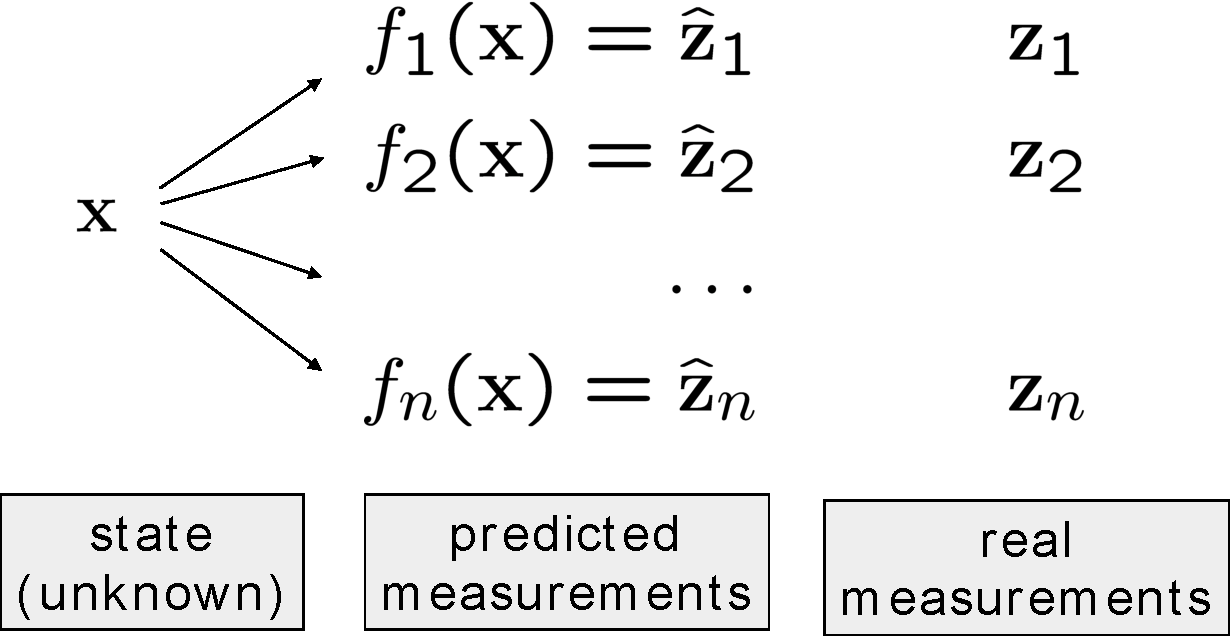
\includegraphics[width=0.7\textwidth]{images/least_squares.pdf}
    \end{center}

\end{frame}

\begin{frame}
    \frametitle{Ejemplo}
    \note{Extraído de Curso de Cyrill Stachniss https://youtu.be/r2cyMQ5NB1o?si=WYODHSkWun3FL7jR}
    
    \begin{center}
        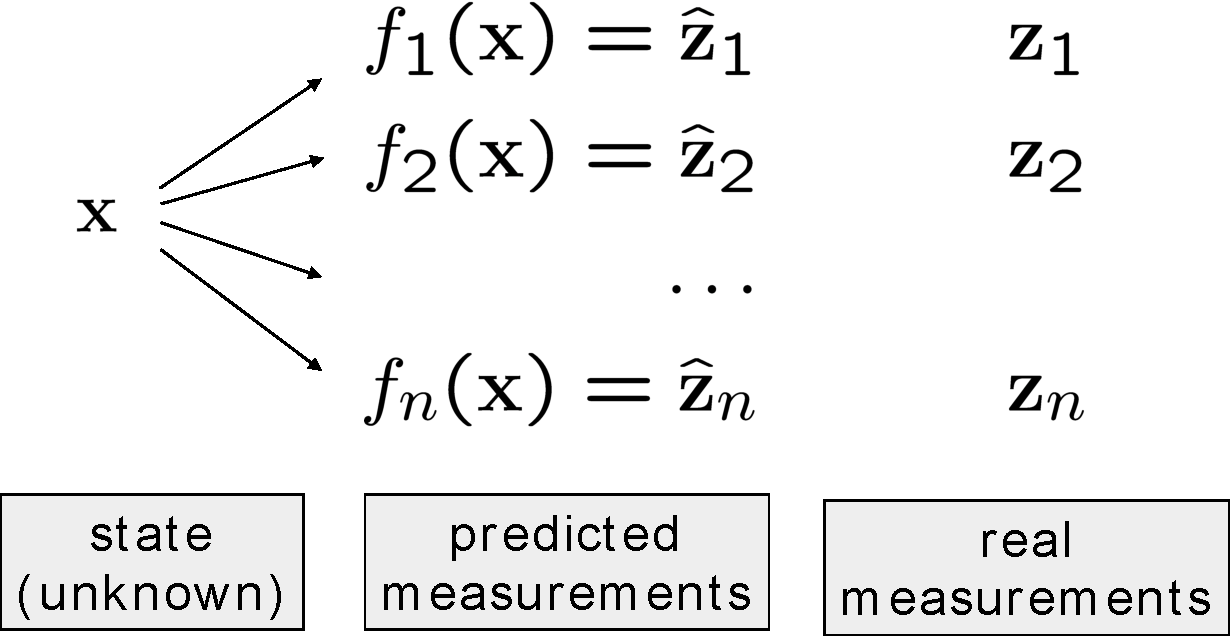
\includegraphics[width=0.7\textwidth]{images/least_squares.pdf}
    \end{center}
    
    \begin{itemize}
        \item $\stateBold$ posición de los puntos 3D
        \item $\observationBold_{i}$ coordenadas de los puntos 3D proyectados en las imágenes
        \item Estimar la posición 3D más probable de los puntos basado en las proyecciones en las imágenes (dada las poses de la cámara)
    \end{itemize}
\end{frame}

\begin{frame}
    \frametitle{Función de Error}
    \note{Extraído de Curso de Cyrill Stachniss https://youtu.be/r2cyMQ5NB1o?si=WYODHSkWun3FL7jR}
    
    \begin{itemize}
        \item El error $\error_{i}$ suele ser la diferencia entre la medición real y la predicción:
            \begin{equation*}
                \error_{i}\left( \stateBold \right) = \observationBold_{i} - f_{i}\left( \stateBold \right)
            \end{equation*}
        \item Supongamos que el error tiene una distribución normal con media cero
        \item Error Gaussiano con matriz de información $\informationMatrix_{i}$
        \item El error al cuadrado de una medición depende sólo del estado y es un escalar:
            \begin{equation*}
                \error_{i}\left( \stateBold \right) = \error_{i}\left( \stateBold \right)^{\top} \informationMatrix_{i} \error_{i}\left( \stateBold \right)
            \end{equation*}
    \end{itemize}
\end{frame}

\begin{frame}
    \frametitle{Objetivo: Encontrar el Mínimo}
    \note{Extraído de Curso de Cyrill Stachniss https://youtu.be/r2cyMQ5NB1o?si=WYODHSkWun3FL7jR}
    
    \begin{itemize}
        \item Encontrar el estado $\stateBold^{*}$ que minimiza el error dados todas las mediciones
        
        \begin{center}
            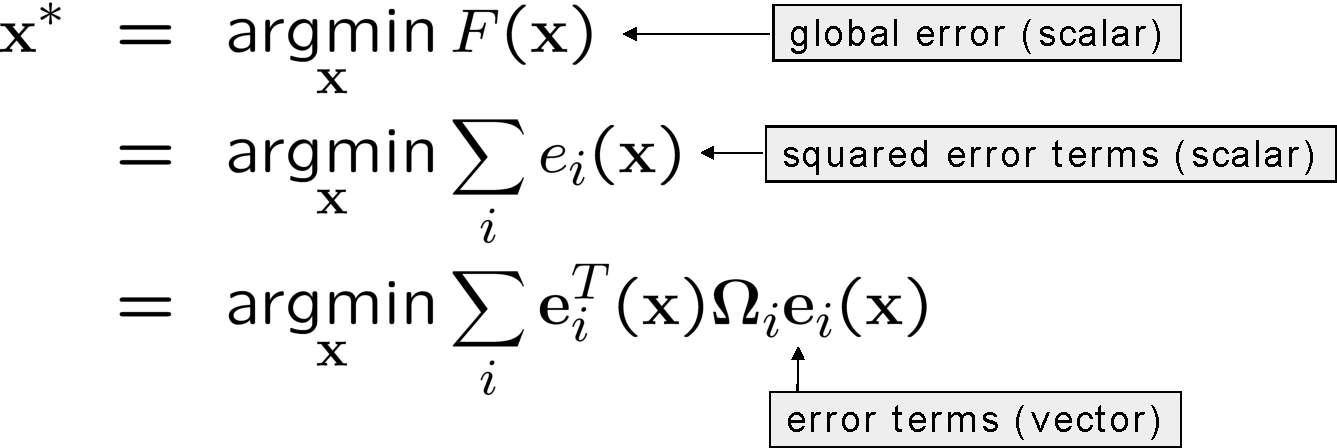
\includegraphics[width=0.7\textwidth]{images/find_minimum.pdf}
        \end{center}
    \end{itemize}

\end{frame}

\begin{frame}
    \frametitle{Objetivo: Encontrar el Mínimo}
    \note{Extraído de Curso de Cyrill Stachniss https://youtu.be/r2cyMQ5NB1o?si=WYODHSkWun3FL7jR}
    
    \begin{itemize}
        \item Encontrar el estado $\stateBold^{*}$ que minimiza el error dados todas las mediciones
        
        \begin{equation*}
            \stateBold^{*} = \argmin_{\stateBold} \sum_{i} \error_{i}\left( \stateBold \right)^{\top} \informationMatrix_{i} \error_{i}\left( \stateBold \right)
        \end{equation*}
        
        
        \item Una solución general es derivar la función de error global y encontrar sus nulos
        \item En general compleja y con solución no cerrada $\rightarrow$ Solución con Métodos numéricos
    \end{itemize}
    
\end{frame}


\begin{frame}
    \frametitle{Suposiciones}
    \note{Extraído de Curso de Cyrill Stachniss https://youtu.be/r2cyMQ5NB1o?si=WYODHSkWun3FL7jR}
    \begin{itemize}
        \item Hay una ``buena'' solución inicial disponible
        \item Las funciones de error son ``suaves'' en la vecindad del mínimo (con suerte global)
        \item Entonces, podemos resolver el problema con linearizaciones locales iterativas
    \end{itemize}

\end{frame}

\begin{frame}
    \frametitle{Resolvemos utilizando Linearizaciones locales iterativas}
    \note{Extraído de Curso de Cyrill Stachniss https://youtu.be/r2cyMQ5NB1o?si=WYODHSkWun3FL7jR}
    \begin{itemize}
        \item Linealizar los términos de error alrededor del solución actual/solución inicial
        \item Calcular la primera derivada de la función de error al cuadrado
        \item Setear en cero y resolver el sistema lineal
        \item Obtener el nuevo estado (que con suerte estará más cerca del mínimo)
        \item Iterar
    \end{itemize}
\end{frame}

\begin{frame}
    \frametitle{Linearizar la Función de Error}
    \note{Extraído de Curso de Cyrill Stachniss https://youtu.be/r2cyMQ5NB1o?si=WYODHSkWun3FL7jR}
    
    \begin{itemize}
        \item Podemos aproximar el error al rededor de una estimación inicial $\stateBold$ a través de una expansión de Taylor
    \end{itemize}
    
    \begin{equation*}
        \error_{i}(\stateBold + \vec{\Delta}\stateBold) \simeq  \underbrace{\error_{i}(\stateBold)}_{\error_{i}} + \jacobian_{i}\vec{\Delta}\stateBold \quad \text{con} \quad \jacobian_{i} = \dfrac{\partial\error_{i}(\stateBold)}{\partial\stateBold}
    \end{equation*}
    
\end{frame}

\begin{frame}
    \frametitle{Error Cuadrático}
    \note{Extraído de Curso de Cyrill Stachniss https://youtu.be/r2cyMQ5NB1o?si=WYODHSkWun3FL7jR}
    
    \begin{itemize}
        \item Con la linealización anterior, podemos fijar $\stateBold$ y llevar a cabo la minimización en los incrementos $\Delta\stateBold$
        \item Reemplazamos la expansión de Taylor en los términos de error al cuadrado:
        \only<1>{
            \begin{align*}
                e_{i}(\stateBold + \vec{\Delta}\stateBold) &= \dots
            \end{align*}
        }
        \only<2>{
            \begin{align*}
                e_{i}(\stateBold + \vec{\Delta}\stateBold) &= \error_{i}\left( \stateBold + \Delta \stateBold \right)^{\top} \informationMatrix_{i} \error_{i}\left( \stateBold  + \Delta \stateBold \right)
            \end{align*}
        }
        \only<3>{
            \begin{align*}
                e_{i}(\stateBold + \vec{\Delta}\stateBold) &= \error_{i}\left( \stateBold + \Delta \stateBold \right)^{\top} \informationMatrix_{i} \error_{i}\left( \stateBold  + \Delta \stateBold \right)\\
                &\simeq \left( \error_{i} + \jacobian_{i} \Delta \stateBold \right)^{\top} \informationMatrix_{i} \left( \error_{i} + \jacobian_{i} \Delta \stateBold \right)
            \end{align*}
        }
        \only<4>{
            \begin{align*}
                e_{i}(\stateBold + \vec{\Delta}\stateBold) &= \error_{i}\left( \stateBold + \Delta \stateBold \right)^{\top} \informationMatrix_{i} \error_{i}\left( \stateBold  + \Delta \stateBold \right)\\
                &\simeq \left( \error_{i} + \jacobian_{i} \Delta \stateBold \right)^{\top} \informationMatrix_{i} \left( \error_{i} + \jacobian_{i} \Delta \stateBold \right)\\
                &= \error_{i}^{\top} \informationMatrix_{i} \error_{i} + \error_{i}^{\top} \informationMatrix_{i} \jacobian_{i} \Delta \stateBold + \Delta \stateBold^{\top} \jacobian_{i}^{\top} \informationMatrix_{i} \error_{i} +  \Delta \stateBold^{\top} \jacobian_{i}^{\top} \informationMatrix_{i} \jacobian_{i} \Delta \stateBold
            \end{align*}
        }
    \end{itemize}
\end{frame}

\begin{frame}
    \frametitle{Error Cuadrático (cont.)}
    \note{Extraído de Curso de Cyrill Stachniss https://youtu.be/r2cyMQ5NB1o?si=WYODHSkWun3FL7jR}
    
    \begin{itemize}
        \item Todos los sumandos son escalares por lo que la transposición no tiene ningún efecto
        \item Agrupando términos similares obtenemos:
        \only<1>{
            \begin{align*}
                e_{i}(\stateBold + \vec{\Delta}\stateBold) &\simeq \error_{i}^{\top} \informationMatrix_{i} \error_{i} + \error_{i}^{\top} \informationMatrix_{i} \jacobian_{i} \Delta \stateBold + \Delta \stateBold^{\top} \jacobian_{i}^{\top} \informationMatrix_{i} \error_{i} +  \Delta \stateBold^{\top} \jacobian_{i}^{\top} \informationMatrix_{i} \jacobian_{i} \Delta \stateBold
            \end{align*}
        }
        \only<2>{
            \begin{align*}
                e_{i}(\stateBold + \vec{\Delta}\stateBold) &\simeq \error_{i}^{\top} \informationMatrix_{i} \error_{i} + \error_{i}^{\top} \informationMatrix_{i} \jacobian_{i} \Delta \stateBold + \Delta \stateBold^{\top} \jacobian_{i}^{\top} \informationMatrix_{i} \error_{i} +  \Delta \stateBold^{\top} \jacobian_{i}^{\top} \informationMatrix_{i} \jacobian_{i} \Delta \stateBold \\
                &= \underbrace{\error_{i}^{\top} \informationMatrix_{i} \error_{i}}_{c_{i}} + 2 \underbrace{\error_{i}^{\top} \informationMatrix_{i} \jacobian_{i}}_{\linearSystemb^{\top}_{i}} \Delta \stateBold + \Delta \stateBold^{\top} \underbrace{\jacobian_{i}^{\top} \informationMatrix_{i} \jacobian_{i}}_{\linearSystemH_{i}} \Delta \stateBold
            \end{align*}
        }
        \only<3>{
            \begin{align*}
                e_{i}(\stateBold + \vec{\Delta}\stateBold) &\simeq \error_{i}^{\top} \informationMatrix_{i} \error_{i} + \error_{i}^{\top} \informationMatrix_{i} \jacobian_{i} \Delta \stateBold + \Delta \stateBold^{\top} \jacobian_{i}^{\top} \informationMatrix_{i} \error_{i} +  \Delta \stateBold^{\top} \jacobian_{i}^{\top} \informationMatrix_{i} \jacobian_{i} \Delta \stateBold \\
                &= \underbrace{\error_{i}^{\top} \informationMatrix_{i} \error_{i}}_{c_{i}} + 2 \underbrace{\error_{i}^{\top} \informationMatrix_{i} \jacobian_{i}}_{\linearSystemb^{\top}_{i}} \Delta \stateBold + \Delta \stateBold^{\top} \underbrace{\jacobian_{i}^{\top} \informationMatrix_{i} \jacobian_{i}}_{\linearSystemH_{i}} \Delta \stateBold \\
                &= c_{i} + 2 \linearSystemb^{\top}_{i} \Delta \stateBold + \Delta \stateBold^{\top} \linearSystemH_{i} \Delta \stateBold
            \end{align*}
        }
    \end{itemize}
    
    
\end{frame}

\begin{frame}
    \frametitle{Error Global}
    \note{Extraído de Curso de Cyrill Stachniss https://youtu.be/r2cyMQ5NB1o?si=WYODHSkWun3FL7jR}
    
    \begin{itemize}
        \item El error global es la suma de términos de errores cuadrados correspondientes a las medidas individuales
        \item Forma una nueva expresión, que se aproxima al error global en la vecindad de la solución actual $\stateBold$
    \end{itemize}
    
    \begin{align*}
        F\left(\stateBold + \Delta \stateBold \right) &= \sum_{i} e_{i}(\stateBold + \vec{\Delta}\stateBold)\\
        F\left(\stateBold + \Delta \stateBold \right) &\simeq \sum_{i} \left( c_{i} + 2 \linearSystemb^{\top}_{i} \Delta \stateBold + \Delta \stateBold^{\top} \linearSystemH_{i} \Delta \stateBold \right) \\
        &= \sum_{i} c_{i} + 2 \left( \sum_{i} \linearSystemb^{\top}_{i} \right) \Delta \stateBold + \Delta \stateBold^{\top} \left( \sum_{i} \linearSystemH_{i} \right) \Delta \stateBold
    \end{align*}
    
    
\end{frame}

\begin{frame}
    \frametitle{Error Global (cont.)}
    \note{Extraído de Curso de Cyrill Stachniss https://youtu.be/r2cyMQ5NB1o?si=WYODHSkWun3FL7jR}
    
    \begin{align*}
        F\left(\stateBold + \Delta \stateBold \right) &\simeq \sum_{i} \left( c_{i} + 2 \linearSystemb^{\top}_{i} \Delta \stateBold + \Delta \stateBold^{\top} \linearSystemH_{i} \Delta \stateBold \right) \\
        &= \underbrace{\sum_{i} c_{i}}_{c} + 2 \underbrace{\left( \sum_{i} \linearSystemb^{\top}_{i} \right)}_{\linearSystemb^{\top}} \Delta \stateBold + \Delta \stateBold^{\top} \underbrace{\left( \sum_{i} \linearSystemH_{i} \right)}_{\linearSystemH} \Delta \stateBold \\
        &= c + 2 \linearSystemb^{\top} \Delta \stateBold + \Delta \stateBold^{\top} \linearSystemH \Delta \stateBold
    \end{align*}
    
    con
    
    \begin{align*}
        \linearSystemb^{\top} &= \sum_{i} \error_{i}^{\top} \informationMatrix_{i} \jacobian_{i} \\ 
        \linearSystemH &= \sum_{i}  \jacobian_{i}^{\top} \informationMatrix_{i} \jacobian_{i}
    \end{align*}
    
    
\end{frame}

\begin{frame}
    \frametitle{Forma Cuadrática}
    \note{Extraído de Curso de Cyrill Stachniss https://youtu.be/r2cyMQ5NB1o?si=WYODHSkWun3FL7jR}
    
    \begin{itemize}
        \item<1-> Podemos escribir los términos de error global como una forma cuadrática en $\Delta \stateBold$
        
        \begin{equation*}
            F\left(\stateBold + \Delta \stateBold \right) = c + 2 \linearSystemb^{\top} \Delta \stateBold + \Delta \stateBold^{\top} \linearSystemH \Delta \stateBold
        \end{equation*}
        
        \item<1> \alert{¿Cómo calcular el mínimo de una forma cuadrática?}
        \item<2-> Calcular la derivada de  $F\left(\stateBold + \Delta \stateBold \right)$ con respecto a $\Delta \stateBold$ (dado $\stateBold$)
        \item<2-> Derivamos e igualamos a 0
        \item<2-> resolvemos
    \end{itemize}

\end{frame}

\begin{frame}
    \frametitle{Derivando la forma cuadrática}
    \note{Extraído de Curso de Cyrill Stachniss https://youtu.be/r2cyMQ5NB1o?si=WYODHSkWun3FL7jR}
    
    \begin{itemize}
        \item Dada la forma cuadrática
        \begin{equation*}
            f(\stateBold) = \stateBold^{\top} \linearSystemH \stateBold + \linearSystemb^{\top} \stateBold
        \end{equation*}
        \item La primera derivada es
        \begin{equation*}
            \dfrac{\partial f}{\partial \stateBold} = \left( \linearSystemH + \linearSystemH^{\top} \right) \stateBold + \linearSystemb
        \end{equation*}
    \end{itemize}
    
    Ver: The Matrix Cookbook, sección 2.4.2
   
\end{frame}

\begin{frame}
    \frametitle{Forma Cuadrática}
    \note{Extraído de Curso de Cyrill Stachniss https://youtu.be/r2cyMQ5NB1o?si=WYODHSkWun3FL7jR}
    
    \begin{itemize}
        \item Podemos escribir los términos de error global de forma cuadrática en $\Delta \stateBold$
        \begin{equation*}
            F\left(\stateBold + \Delta \stateBold \right) = c + 2 \linearSystemb^{\top} \Delta \stateBold + \Delta \stateBold^{\top} \linearSystemH \Delta \stateBold
        \end{equation*}
        \item La derivada de $F\left(\stateBold + \Delta \stateBold \right)$
        \begin{equation*}
            \dfrac{\partial F\left(\stateBold + \Delta \stateBold \right)}{\partial \Delta \stateBold} \simeq 2 \linearSystemb + 2 \linearSystemH \Delta \stateBold
        \end{equation*}
    \end{itemize}
    
\end{frame}

\begin{frame}
    \frametitle{Minimizando la forma cuadrática}
    \note{Extraído de Curso de Cyrill Stachniss https://youtu.be/r2cyMQ5NB1o?si=WYODHSkWun3FL7jR}
    
    \begin{itemize}
        \item Derivada de $F\left(\stateBold + \Delta \stateBold \right)$
        \begin{equation*}
            \dfrac{\partial F\left(\stateBold + \Delta \stateBold \right)}{\partial \Delta \stateBold} \simeq 2 \linearSystemb + 2 \linearSystemH \Delta \stateBold
        \end{equation*}
        \item Igualando a 0
        \begin{equation*}
            0 = 2 \linearSystemb + 2 \linearSystemH \Delta \stateBold
        \end{equation*}
        \item Lo que lleva al sistema lineal
        \begin{equation*}
            \linearSystemH \Delta \stateBold = -\linearSystemb 
        \end{equation*}
        \item La solución para el incremento $\Delta \stateBold^{*}$ es
        \begin{equation*}
             \Delta \stateBold^{*} = - \inverse{\linearSystemH} \linearSystemb 
        \end{equation*}
    \end{itemize}
    
\end{frame}

\begin{frame}
    \frametitle{Solución con Gauss-Newton}
    \note{Extraído de Curso de Cyrill Stachniss https://youtu.be/r2cyMQ5NB1o?si=WYODHSkWun3FL7jR}
    
    Iterar los siguientes pasos:
    \begin{itemize}
        \item Lineanizar cerca de $\stateBold$ y computar para cada medición
        \begin{equation*}
            \error_{i}(\stateBold + \vec{\Delta}\stateBold) \simeq  \error_{i}(\stateBold) + \jacobian_{i}\vec{\Delta}\stateBold
        \end{equation*}
        \item Computar los términos del sistema lineal
        \begin{equation*}
            \linearSystemb^{\top} = \sum_{i} \error_{i}^{\top} \informationMatrix_{i} \jacobian_{i} \quad \quad \linearSystemH = \sum_{i} \jacobian_{i}^{\top} \informationMatrix_{i} \jacobian_{i}
        \end{equation*}
    \item Resolver el sistema lineal
    \begin{equation*}
        \Delta \stateBold^{*} = - \inverse{\linearSystemH} \linearSystemb 
    \end{equation*}
    \item Actualizar el estado
    \begin{equation*}
        \stateBold \leftarrow \stateBold + \Delta \stateBold^{*}
    \end{equation*} 
    \end{itemize}
    
\end{frame}

\begin{frame}
    \frametitle{Ejemplo: Calibración de Odometría}
    \note{Extraído de Curso de Cyrill Stachniss https://youtu.be/r2cyMQ5NB1o?si=WYODHSkWun3FL7jR}
    
    \begin{itemize}
        \item Mediciones de Odometría $\controlCommand_{i}$
        \item Eliminar el error sistemático a través de la calibración
        \item Suposición: disponemos del ground-truth de odometría $\controlCommand_{i}^{*}$
        \item Ground-truth dado por sistemas: Motion Capture (Vicon), Scan-Matching o SLAM
    \end{itemize}
    
\end{frame}

\begin{frame}
    \frametitle{Ejemplo: Calibración de Odometría}
    \note{Extraído de Curso de Cyrill Stachniss https://youtu.be/r2cyMQ5NB1o?si=WYODHSkWun3FL7jR}
    
    \begin{itemize}
        \item Hay una función que $f_{i}(\stateBold)$ que dado algunos parámetros de bias $\stateBold$, devuelve una odometría corregida (\emph{unbiased}) para la lectura ruidosa $\controlCommand_{i}^{\prime}$ 
        \begin{equation*}
            \controlCommand_{i}^{\prime} = f_{i}(\stateBold) =
            \begin{bmatrix}
                x_{11} & x_{12} & x_{13} \\
                x_{21} & x_{22} & x_{23} \\
                x_{31} & x_{32} & x_{33}
            \end{bmatrix}
            \controlCommand_{i}
        \end{equation*}
    \item Para obtener la función de corrección $f(\stateBold)$, necesitamos encontrar los parámetros $\stateBold$
    \end{itemize}
    
\end{frame}

\begin{frame}
    \frametitle{Calibración de Odoemtría (cont.)}
    \note{Extraído de Curso de Cyrill Stachniss https://youtu.be/r2cyMQ5NB1o?si=WYODHSkWun3FL7jR}
    \begin{itemize}

        \item El vector estado es 
        \begin{equation*}
            \stateBold =
            \begin{bmatrix}
                x_{11} & x_{12} & x_{13} & x_{21} & x_{22} & x_{23} & x_{31} & x_{32} & x_{33}
            \end{bmatrix}
        \end{equation*}
        \item La función error es
        \begin{equation*}
            \error_{i}(\stateBold) = \controlCommand_{i}^{*} - 
            \begin{bmatrix}
                x_{11} & x_{12} & x_{13} \\
                x_{21} & x_{22} & x_{23} \\
                x_{31} & x_{32} & x_{33}
            \end{bmatrix}
            \controlCommand_{i}
        \end{equation*}
        \item Su derivada es
        
    %    \begin{equation*}
    %        \jacobian_{i} = \dfrac{\partial \error_{i}(\stateBold)}{\partial \stateBold} = -
    %        \begin{bmatrix}
    %            u_{i,x} & u_{i,y} & u_{i,\theta} & 0 & 0 & 0 & 0 & 0 & 0 \\
    %            0 & 0 & 0 & u_{i,x} & u_{i,y} & u_{i,\theta} & 0 & 0 & 0 \\
    %            0 & 0 & 0 & 0 & 0 & 0 & u_{i,x} & u_{i,y} & u_{i,\theta}
    %        \end{bmatrix}
    %    \end{equation*}
    
        \begin{center}
            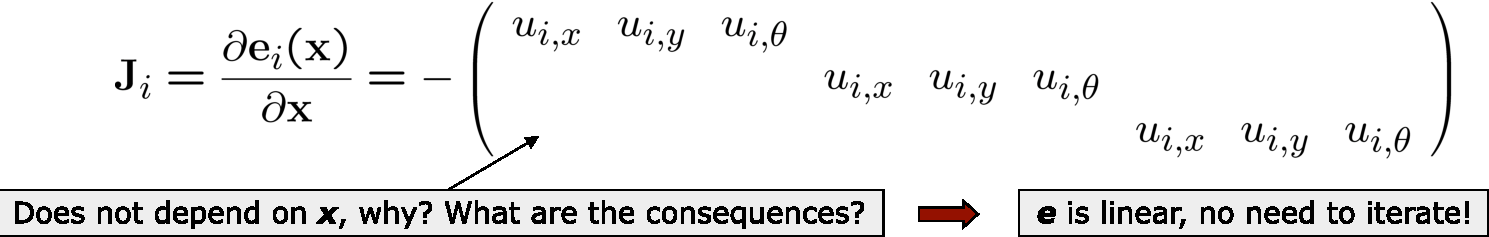
\includegraphics[width=0.8\columnwidth]{images/odometry_calibration_jacobian.pdf}
        \end{center}
        
        Que la primera derivada (Jacobiano) no dependa de $\stateBold$, es lo menos común, ya que significa que la función $\error$ es lineal!
        
        En este caso solo vamos a tener que hacer una sola iteración.

    \end{itemize}

    
\end{frame}

\begin{frame}
    \frametitle{Preguntas}
    \note{Extraído de Curso de Cyrill Stachniss https://youtu.be/r2cyMQ5NB1o?si=WYODHSkWun3FL7jR}
    
    \begin{itemize}
        \item<1-> ¿Cómo lucen los parámetros si la odometría es perfecta?
        \begin{itemize}
            \item<2-> La matriz debería ser la identidad. Entonces el error es 0, y por lo tanto, encontramos el mínimo.
        \end{itemize}
        \item<3-> ¿Cuantas mediciones son necesarias para encontrar la solución al problema de calibración?
        \begin{itemize}
            \item<4-> Tenemos que ver cuantas variables desconocidas tenemos y cuanta información nos provee cada observación. Tenemos 9 variables desconocidas. Cada observación nos da información de 3 variables (nos da 3 ecuaciones). Por lo tanto, vamos a necesitar al menos 3 observaciones.
        \end{itemize}
        \item<5-> $\linearSystemH$ es simétrica. ¿Por qué?
        \begin{itemize}
            \item<6-> La forma en que $\linearSystemH$ es simétrica porque  $\linearSystemH = \jacobian^{\top}\Omega\jacobian$. $\Omega$ es simétrica definida postiva y $\jacobian$ tambien, y por lo tanto el producto también.
        \end{itemize}
        \item<7-> ¿Cómo afecta la estructura de la función de medición a la estructura de $\linearSystemH$?
        \begin{itemize}
            \item<8-> $\linearSystemH$ es esparsa porque los jacobianos son esparsos. Los jacobianos son esparsos porque codifican cuanta información nos da una medición sobre todas las variables de estado. Por lo tanto, si nuestras mediciones solo relacionan algunas variables (como es el caso de SLAM), entonces la $\linearSystemH$ será esparsa.
        \end{itemize}
    \end{itemize}

\end{frame}

\begin{frame}
    \frametitle{¿Cómo Resolver de manera eficiente un Sistema Lineal?}
    \note{Extraído de Curso de Cyrill Stachniss https://youtu.be/r2cyMQ5NB1o?si=WYODHSkWun3FL7jR}
    \begin{itemize}
        \item Sistema Lineal $\linearSystemH \Delta \stateBold = -\linearSystemb$
        \item Podemos resolverlo utilizando inversión de matrices (en teoría)
        \item En la práctica:
        \begin{itemize}
            \item Factorización de Cholesky
            \item Descomposición QR
            \item Métodos iterativos como el método del Gradiente Conjugado (para sistemas grandes)
        \end{itemize}
        
    \end{itemize}
    
\end{frame}

\begin{frame}
    \frametitle{Descomposición de Cholesky para Resolver un Sistema Lineal}
    \note{Extraído de Curso de Cyrill Stachniss https://youtu.be/r2cyMQ5NB1o?si=WYODHSkWun3FL7jR}
    
    \begin{itemize}
        \item Sea la matriz $\vec{A}$ simétrica positiva definida
        \item El sistema a resolver es $\vec{A} \vec{x} = \vec{b}$
        \item Cholesky lleva a $\vec{A} = \vec{L} \vec{L}^{\top}$ con $\vec{L}$ matriz triangular inferior
        \item<2> Resolvemos primero
        \begin{equation*}
            \vec{L} \vec{y} = \vec{b}
        \end{equation*}
        \item<2> y luego,
        \begin{equation*}
            \vec{L}^{\top} \vec{x} = \vec{y}
        \end{equation*}
    
    \end{itemize}
    
\end{frame}

\begin{frame}
    \frametitle{Resumen de Gauss-Newton}
    \note{Extraído de Curso de Cyrill Stachniss https://youtu.be/r2cyMQ5NB1o?si=WYODHSkWun3FL7jR}
    
    Método para minimizar un error al cuadrado:
    \begin{itemize} 
        \item Comenzar con una solución inicial (\emph{initial guess})
        \item Linealizar las funciones de error individuales
        \item Esto lleva a una forma cuadrática
        \item Se obtiene un sistema lineal derivando e igualando a 0
        \item Resolver el sistema lineal conduce a una actualización del estado
        \item Iterar
    \end{itemize}
    
\end{frame}

\begin{frame}
    \frametitle{Least Squares vs. Probabilistic State Estimation}
    \note{Extraído de Curso de Cyrill Stachniss https://youtu.be/r2cyMQ5NB1o?si=WYODHSkWun3FL7jR}
    
    \begin{itemize}
        \item Hasta ahora, minimizamos una función de error
        \item ¿Cómo se relaciones esto con la estimación de estado en el sentido probabilístico?
    \end{itemize}
    
\end{frame}

\begin{frame}
    \frametitle{Comencemos con Estimación de estado}
    \note{Extraído de Curso de Cyrill Stachniss https://youtu.be/r2cyMQ5NB1o?si=WYODHSkWun3FL7jR}
    
    \begin{itemize}
        \item Regla de Bayes, suposiciones de independencia y Markov nos permiten reescribir
        \begin{equation*}
            p\left( \state_{0:t} | \observation_{1:t}, \controlCommand_{1:t} \right) = \eta p\left( \state_{0} \right) \prod_{t} \left[ p\left( \state_{t} | \state_{t-1}, \controlCommand_{t} \right) p\left( \observation_{t} | \state_{t} \right) \right]
        \end{equation*}
    \end{itemize}
    
    \note{p(x0) es un prior. Observar que en x0 no tenemos observaciones ni comandos de control}
    
\end{frame}

\begin{frame}
    \frametitle{Log Likelihood}
    \note{Extraído de Curso de Cyrill Stachniss https://youtu.be/r2cyMQ5NB1o?si=WYODHSkWun3FL7jR}
    
    \begin{itemize}
        \item Reescribiendo como el log likelihood, lleva a
        \begin{equation*}
            \log p\left( \state_{0:t} | \observation_{1:t}, \controlCommand_{1:t} \right) = \text{const.}  \log p\left( \state_{0} \right) + \sum_{t} \left[ \log p\left( \state_{t} | \state_{t-1}, \controlCommand_{t} \right) + \log p\left( \observation_{t} | \state_{t} \right) \right]
        \end{equation*}
    \end{itemize}
    
\end{frame}

\begin{frame}
    \frametitle{Suposición Gaussiana}
    \note{Extraído de Curso de Cyrill Stachniss https://youtu.be/r2cyMQ5NB1o?si=WYODHSkWun3FL7jR}
    
    \begin{itemize}
        \item Suponiendo distribución Gaussiana
        \begin{equation*}
            \log p\left( \state_{0:t} | \observation_{1:t}, \controlCommand_{1:t} \right) = \text{const.}  \log \underbrace{p\left( \state_{0} \right)}_{\mathcal{N}} + \sum_{t} \left[ \log \underbrace{p\left( \state_{t} | \state_{t-1}, \controlCommand_{t} \right)}_{\mathcal{N}} + \log \underbrace{p\left( \observation_{t} | \state_{t} \right)}_{\mathcal{N}} \right]
        \end{equation*}
    \end{itemize}
    
\end{frame}

\begin{frame}
    \frametitle{Log de una Gaussiana}
    \note{Extraído de Curso de Cyrill Stachniss https://youtu.be/r2cyMQ5NB1o?si=WYODHSkWun3FL7jR}

    
    \begin{itemize}
        \item La función de distribución de la distribución normal está definida como
        \begin{equation*}
            p(x)=\det(2\pi\covariance)^{\frac{1}{2}} \exp\left(-\dfrac{1}{2} (x - \mu )^{\top} \inverse{\covariance} (x - \mu )  \right)
        \end{equation*}
        
        \item Log likelihood de una Gaussiana
        \begin{equation*}
            \log \mathcal{N}(x, \mu, \Sigma) =  \text{const.} - \dfrac{1}{2} (x - \mu)^{\top} \inverse{\Sigma} (x - \mu)
        \end{equation*}
    \end{itemize}
    
\end{frame}

\begin{frame}
    \frametitle{Función de Error como Exponente}
    \note{Extraído de Curso de Cyrill Stachniss https://youtu.be/r2cyMQ5NB1o?si=WYODHSkWun3FL7jR}
    
    \begin{itemize}
        \item Log likelihood de una Gaussiana
        \begin{equation*}
            \log \mathcal{N}(x, \mu, \Sigma) =  \text{const.} - \dfrac{1}{2} \underbrace{\underbrace{(x - \mu)^{\top}}_{\error^{\top}(x)} \underbrace{\inverse{\Sigma}}_{\informationMatrix} \underbrace{(x - \mu)}_{\error(x)}}_{e(x)}
        \end{equation*}
        \item está a una constante de equivalencia de las funciones de error usadas antes
    \end{itemize}
    
\end{frame}

\begin{frame}
    \frametitle{Log Likelihood con Términos de Error}
    \note{Extraído de Curso de Cyrill Stachniss https://youtu.be/r2cyMQ5NB1o?si=WYODHSkWun3FL7jR}
    
    \begin{itemize}
        \item Suponiendo distribución Gaussiana
        \begin{equation*}
            \log p\left( \state_{0:t} | \observation_{1:t}, \controlCommand_{1:t} \right) = \text{const.} - \dfrac{1}{2} e_{p}(\state) -  \dfrac{1}{2} \sum_{t} \left[ e_{\controlCommand_{t}}(\state) + e_{\observation_{t}}(\state)\right]
        \end{equation*}
    \end{itemize}
    
\end{frame}

\begin{frame}
    \frametitle{Maximizing el Log Likelihood}
    \note{Extraído de Curso de Cyrill Stachniss https://youtu.be/r2cyMQ5NB1o?si=WYODHSkWun3FL7jR}
    
    \begin{itemize}
        \item Suponiendo distribución Gaussiana
        \begin{equation*}
            \log p\left( \state_{0:t} | \observation_{1:t}, \controlCommand_{1:t} \right) = \text{const.} - \dfrac{1}{2} e_{p}(\state) -  \dfrac{1}{2} \sum_{t} \left[ e_{\controlCommand_{t}}(\state) + e_{\observation_{t}}(\state)\right]
        \end{equation*}
        \item Maximizando el log likelihood lleva a 
        \begin{equation*}
            \argmax \log p\left( \state_{0:t} | \observation_{1:t}, \controlCommand_{1:t} \right) = \argmin e_{p}(\state) + \sum_{t} \left[ e_{\controlCommand_{t}}(\state) + e_{\observation_{t}}(\state)\right]
        \end{equation*}
    \end{itemize}
    
    
\end{frame}

\begin{frame}
    \frametitle{Minimizar el error cuadrático es equivalente a Maximizar el Log Likelihood de Distribuciones Gaussianas Independientes}
    \note{Extraído de Curso de Cyrill Stachniss https://youtu.be/r2cyMQ5NB1o?si=WYODHSkWun3FL7jR}
    \begin{itemize}
        \item Con términos de error individuales para los controles, mediciones y un prior:
        \begin{equation*}
            \argmax \log p\left( \state_{0:t} | \observation_{1:t}, \controlCommand_{1:t} \right) = \argmin e_{p}(\state) + \sum_{t} \left[ e_{\controlCommand_{t}}(\state) + e_{\observation_{t}}(\state)\right]
        \end{equation*}
    \end{itemize}
    
\end{frame}

\begin{frame}
    \frametitle{Resumen}
    \note{Extraído de Curso de Cyrill Stachniss https://youtu.be/r2cyMQ5NB1o?si=WYODHSkWun3FL7jR}
    
    \begin{itemize}
        \item Técnica para minimizar funciones de error cuadráticas
        \item Gauss-Newton es un enfoque iterativo para problemas no lineales
        \item Utiliza linearización (¡aproximación!)
        \item Equivalente a maximizar el log likelihood de Gaussianas independientes
        \item Método popular en muchas disciplinas.
    \end{itemize}

    
\end{frame}

\begin{frame}
    \frametitle{Bibliografía de Gauss-Newton}
    \note{Extraído de Curso de Cyrill Stachniss https://youtu.be/r2cyMQ5NB1o?si=WYODHSkWun3FL7jR}
    \begin{itemize}
        \item Capítulo 11.4 de \cite{thrun2005probabilistic}
    \end{itemize}
\end{frame}
    
    \begin{frame}
    \frametitle{Error Function}
    \note{Information taken from https://youtu.be/uHbRKvD8TWg}
    
    \begin{itemize}
    \item Error Function for a Single Constraint
    \begin{figure}
    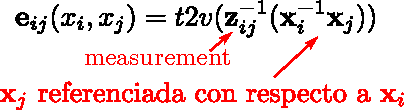
\includegraphics[width=0.44\textwidth]{pose_graph_error_function.pdf}
    \end{figure}
    \footnotetext{$t2v(.)$ maps transformations to vectors}
    
    \item Error as a Function of a Full State Vector
    
    \begin{equation*}
    \error_{ij}(\state) = t2v(\inverse{\observationBold}_{ij}(\inverse{\stateBold}_{i}\stateBold_{j}))
    \end{equation*}
    
    \item The error takes the value 0 when
    
    \begin{equation*}
    \observationBold_{ij} = (\inverse{\stateBold}_{i}\stateBold_{j})
    \end{equation*}
    
    \end{itemize}
    \end{frame}
    
    \begin{frame}
    \frametitle{Linearizing the error function}
    \note{Information taken from https://youtu.be/uHbRKvD8TWg}
    
    \begin{itemize}
    \item We can approximate the error around an initial estimate $\stateBold$ through a Taylor expansion
    \end{itemize}
    
    \begin{equation*}
    \error_{ij}(\stateBold + \vec{\Delta}\stateBold) \simeq \error_{ij}(\stateBold) + \jacobian_{ij}\vec{\Delta}\stateBold \quad \text{con} \quad \jacobian_{ij} = \dfrac{\partial\error_{ij}(\stateBold)}{\partial\stateBold}
    \end{equation*}
    
    \end{frame}
    
    \begin{frame}
    \frametitle{Derivative of the error function}
    \note{Information taken from https://youtu.be/uHbRKvD8TWg}
    \begin{itemize}
    \item<1-> Question: Does an error term $\error_{ij}(\stateBold)$ depend on all state variables?
    
    \only<2->{No, it only depends on $\stateBold_{i}$ and $\stateBold_{j}$}
    
    \item<3-> Question: Are there any consequences for the structure of the Jacobian?
    
    \only<4->{
     Yes, it will be different from zero only in the rows corresponding to $\stateBold_{i}$ and $\stateBold_{j}$
    
     \begin{align*}
     \dfrac{\partial\error_{ij}(\stateBold)}{\partial\stateBold} &=
     \begin{bmatrix}
     0 & \dots & \dfrac{\partial\error_{ij}(\stateBold_{i})}{\partial\stateBold_{i}} & \dots & 0 & \dots & \dfrac{\partial\error_{ij}(\stateBold_{j})}{\partial\stateBold_{j}} & \dots & 0
     \end{bmatrix} \\
     \jacobian_{ij} &=
     \begin{bmatrix}
     0 & \dots & \vec{A}_{ij} & \dots & 0 & \dots & \vec{B}_{ij} & \dots & 0
     \end{bmatrix}
     \end{align*}
     }
    
    
     \end{itemize}
    
    \end{frame}
    
    
    \begin{frame}
     \frametitle{Jacobians and the sparse problem}
     \note{Information taken from https://youtu.be/uHbRKvD8TWg}
    
     \begin{itemize}
     \item The error $\error_{ij}(\stateBold)$ depends only on the parameter blocks $\stateBold_{i}$ and $\stateBold_{j}$
    
     \begin{equation*}
     \error_{ij}(\stateBold) =\error_{ij}(\stateBold_{i} ,\stateBold_{j})
     \end{equation*}
    
     \item The Jacobian will be zero everywhere except in the columns $\stateBold_{i}$ and $\stateBold_{j}$
    
     \begin{equation*}
     \jacobian_{ij} =
     \begin{bmatrix}
     0 & \dots & 0 & \dfrac{\partial\error_{ij}(\stateBold_{i})}{\partial\stateBold_{i}} & 0 & \dots & 0 & \dfrac{\partial\error_{ij}(\stateBold_{j})}{\partial\stateBold_{j}} & 0 & \dots & 0
     \end{bmatrix}
     \end{equation*}
    
     \end{itemize}
    
     {\bf This allows us to solve SLAM efficiently!}
    
\end{frame}


\begin{frame}
    \frametitle{Consequence of this being a sparse problem}
    \note{Information taken from https://youtu.be/uHbRKvD8TWg}
    
    \begin{itemize}
    \item We need to compute the coefficient vector.
    \begin{align*}
    \linearSystemb^{\top} &= \sum_{ij} \linearSystemb_{ij}^{\top} = \sum_{ij} \error_{ij}^{\top}\Omega_{ij}\jacobian_{ij}\\
    \linearSystemH &= \sum_{ij} \linearSystemH_{ij} = \sum_{ij} \jacobian_{ij}^{\top}\Omega_{ij}\jacobian_{ij}
    \end{align*}
    \item The sparse structure of $\jacobian_{ij}$ will result in a sparse structure of $\linearSystemH$
    \item This structure reflects the graph's adjacency matrix.
    \end{itemize}
    
    \end{frame}
    
    \begin{frame}
    \frametitle{Illustration of the structure}
    \note{Information taken from https://youtu.be/uHbRKvD8TWg}
    
    \begin{figure}[!h]
    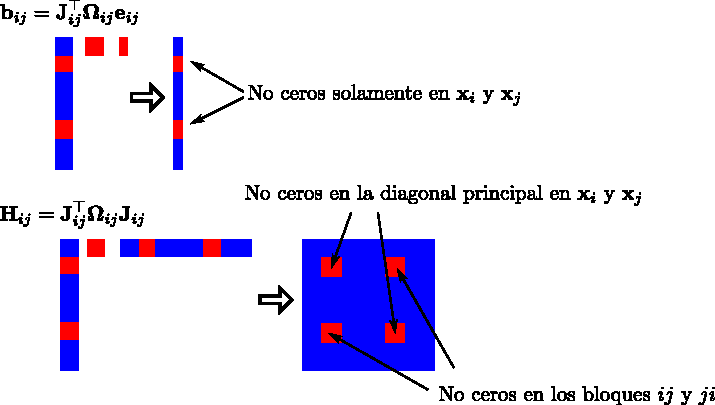
\includegraphics[width=0.9\textwidth]{linear_system_sparsity.pdf}
    \end{figure}
    
    \end{frame}
    
    \begin{frame}
    \frametitle{Consequence of it being a sparse problem}
    \note{Information taken from https://youtu.be/uHbRKvD8TWg}
    
    \begin{figure}[!h]
    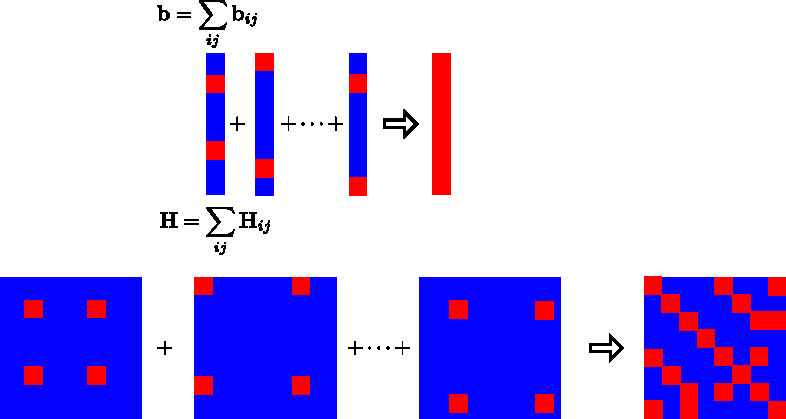
\includegraphics[width=0.9\textwidth]{linear_system_sparsity2.pdf} 
    \end{figure}
    
    \end{frame}
    
    \begin{frame}
     \frametitle{Consequence of it being a dispersed problem}
     \note{Information taken from https://youtu.be/uHbRKvD8TWg}
    
     \begin{itemize}
     \item An edge contributes to the linear system through $\linearSystemb_{ij}$ and $\linearSystemH_{ij}$
     \item The coefficient vector is
    
     \begin{align*}
     \linearSystemb_{ij}^{\top} &= \error_{ij}^{\top}\informationMatrix_{ij}\jacobian_{ij}\\
     &= \error_{ij}^{\top}\informationMatrix_{ij}
     \begin{bmatrix}
     0 & \dots & \vec{A}_{ij} & \dots & \vec{B}_{ij} & \dots & 0
    \end{bmatrix}\\
    &=
    \begin{bmatrix}
    0 & \dots & \error_{ij}^{\top}\informationMatrix_{ij}\vec{A}_{ij} & \dots & \error_{ij}^{\top}\informationMatrix_{ij}\vec{B}_{ij} & \dots & 0
    \end{bmatrix}
    \end{align*}
    \item It is nonzero only at the corresponding indices of $\stateBold_{i}$ and $\stateBold_{j}$
    \end{itemize}
    
    \end{frame}
    
    \begin{frame}
    \frametitle{Consequence of it being a sparse problem}
    \note{Information taken from https://youtu.be/uHbRKvD8TWg}
    \small
    \begin{itemize}
    \item The coefficient matrix of an edge is
     \begin{align*}
     \linearSystemH_{ij}^{\top} &= \jacobian_{ij}^{\top}\informationMatrix_{ij}\jacobian_{ij}\\
     &=
     \begin{bmatrix}
     \vdots \\
     \vec{A}_{ij}^{\top}\\
     \vdots \\
     \vec{B}_{ij}^{\top}\\
     \vdots
     \end{bmatrix} \informationMatrix_{ij}
     \begin{bmatrix}
     \cdots & \vec{A}_{ij} & \cdots & \vec{B}_{ij} & \cdots
     \end{bmatrix}\\
     &=
     \begin{bmatrix}
     0 & \cdots & 0 & \cdots & 0 \\
     \vdots & \vec{A}_{ij}^{\top}\informationMatrix_{ij}\vec{A}_{ij} & \vdots & \vec{A}_{ij}^{\top}\informationMatrix_{ij}\vec{B}_{ij} & \vdots\\
     0 & \cdots & 0 & \cdots & 0 \\
     \vdots & \vec{B}_{ij}^{\top}\informationMatrix_{ij}\vec{A}_{ij} & \vdots & \vec{B}_{ij}^{\top}\informationMatrix_{ij}\vec{B}_{ij} & \vdots\\
     0 & \cdots & 0 & \cdots & 0
     \end{bmatrix}
     \end{align*}
     \item Is non-zero in related blocks with $i,j$
    \end{itemize}
    
    \end{frame}
    
    \begin{frame}
    \frametitle{Summary of the sparse problem}
    \note{Information taken from https://youtu.be/uHbRKvD8TWg}
    
    \begin{itemize}
    \item An edge ij only contributes to
    \begin{itemize}
    \item the i-th and j-th blocks of $\linearSystemb_{ij}$
    \item the blocks $ii$, $jj$, $ij$, and $ji$ of $\linearSystemH_{ij}$
    \end{itemize}
    \item The resulting system is sparse.
    \item The system can be computed by summing the contributions of each edge.
    \item Different \emph{solvers} can be used.
    \begin{itemize}
    \item Sparse Cholesky decomposition.
    \item Conjugate gradient. \item many more...
     \end{itemize}
    
     \end{itemize}
    
    
\end{frame}

\begin{frame}
    \frametitle{The Linear System}
    \note{Information taken from https://youtu.be/uHbRKvD8TWg}
   
    \begin{itemize}
    \item Vector of state increments
    \begin{equation*}
    \Delta\stateBold^{\top} =
    \begin{bmatrix}
    \Delta\stateBold_{1}^{\top} & \Delta\stateBold_{2}^{\top} & \cdots & \Delta\stateBold_{n}^{\top}
    \end{bmatrix}
    \end{equation*}
    \item Coefficient vector
    \begin{equation*}
    \linearSystemb^{\top} =
    \begin{bmatrix}
    \overline{\linearSystemb}_{1}^{\top} & \overline{\linearSystemb}_{2}^{\top} & \cdots & \overline{\linearSystemb}_{n}^{\top}
    \end{bmatrix}
    \end{equation*}
    \item Matrix of normal equations
    \begin{equation*}
    \linearSystemH =
    \begin{bmatrix}
    \overline{\linearSystemH}_{11} & \overline{\linearSystemH}_{12} & \cdots & \overline{\linearSystemH}_{1n}\\
    \overline{\linearSystemH}_{21} & \overline{\linearSystemH}_{22} & \cdots & \overline{\linearSystemH}_{2n}\\
    \vdots & \vdots & \ddots & \vdots\\
    \overline{\linearSystemH}_{n1} & \overline{\linearSystemH}_{n2} & \cdots & \overline{\linearSystemH}_{nn}\\
   \end{bmatrix}
   \end{equation*}
   \end{itemize}
   
   \end{frame}
   
   \begin{frame}
   \frametitle{Construction of the linear system}
   \note{Information taken from https://youtu.be/uHbRKvD8TWg}
   For each constraint:
   \begin{itemize}
   \item Compute the error $\error_{ij} = t2v(\inverse{\observationBold}_{ij}(\inverse{\stateBold}_{i}\stateBold_{j}))$
   \item Compute the blocks of the Jacobians:
   \begin{equation*}
   \vec{A}_{ij} = \dfrac{\partial\error _{ij}(\stateBold _{i}, \stateBold _{j})}{\partial\stateBold _{i}} \quad \quad \vec{B}_{ij} = \dfrac{\partial\error _{ij}(\stateBold _{i}, \stateBold _{j})}{\partial\stateBold _{j}}
    \end{equation*}
    \item Update the coefficient vector:
    \begin{equation*}
    \overline{\linearSystemb}_{i}^{\top} += \error_{ij}^{\top}\informationMatrix_{ij}\vec{A}_{ij} \quad \quad \overline{\linearSystemb}_{j}^{\top} += \error_{ij}^{\top}\informationMatrix_{ij}\vec{B}_{ij}
    \end{equation*}
   
    \item Update the coefficient vector:
    \begin{align*}
    \overline{\linearSystemH}_{ij}^{\top} &+= \vec{A}_{ij}^{\top}\informationMatrix_{ij}\vec{A}_{ij} \quad \quad \overline{\linearSystemH}_{ij}^{\top} += \vec{A}_{ij}^{\top}\informationMatrix_{ij}\vec{B}_{ij} \\
    \overline{\linearSystemH}_{ij}^{\top} &+= \vec{B}_{ij}^{\top}\informationMatrix_{ij}\vec{A}_{ij} \quad \quad \overline{\linearSystemH}_{ij}^{\top} += \vec{B}_{ij}^{\top}\informationMatrix_{ij}\vec{B}_{ij}
    \end{align*}
    \end{itemize}
   
   \end{frame}
   
   \begin{frame}
    \frametitle{Algorithm}
    \note{Information taken from https://youtu.be/uHbRKvD8TWg}
   
    \begin{algorithmic}[1]
    \Procedure{optimize}{$\stateBold$}
    \While (!converged)
    \State $(\linearSystemH,\linearSystemb) = buildLinearSystem(\stateBold)$
    \State $\vec{\Delta}\stateBold = solveSparse(\linearSystemH\vec{\Delta}\stateBold = -\linearSystemb)$
    \State $\stateBold = \stateBold + \vec{\Delta}\stateBold$
    \EndWhile
   
    \State \Return $\stateBold$
    \EndProcedure
    \end{algorithmic}
   
   \end{frame}
   
   
   \begin{frame}
    \frametitle{1D Trivial Example}
    \note{Information taken from https://youtu.be/uHbRKvD8TWg}
   
    Two nodes and one observation
   
    \begin{figure}[!h]
    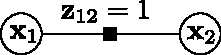
\includegraphics[width=0.2\textwidth]{pose_graph_1d_example.pdf}
    \end{figure}
   
    \small
   
    \begin{align*}
    \stateBold &=
    \begin{bmatrix}
    \stateBold_{1} & \stateBold_{2}
    \end{bmatrix}^{\top}
    =
    \begin{bmatrix}
    0 & 0
    \end{bmatrix}\\
    \observationBold_{12} &= 1\\
    \informationMatrix_{12} &= 2\\
    \error_{12} &= \observationBold_{12} - (\stateBold_{2} - \stateBold_{1}) = 1 - (0 - 0) = 1\\
    \jacobian_{12} &=
    \begin{bmatrix}
    1 & -1
    \end{bmatrix}\\
    \linearSystemb_{12}^{\top} &= \error_{12}^{\top} \informationMatrix_{12} \jacobian_{12} =
    \begin{bmatrix}
    2 & -2
    \end{bmatrix}\\
    \linearSystemH_{12} &= \jacobian_{12}^{\top} \informationMatrix_{12} \jacobian_{12} =
    \begin{bmatrix}
    2 & -2\\
    -2 & 2
    \end{bmatrix}\\
    \vec{\Delta}\stateBold &= -\inverse{\linearSystemH}_{12} \linearSystemb_{12}\\
    \end{align*}
   
    \begin{center}
    \alert{Problem:} $\det(\linearSystemH) = 0$, therefore we cannot invert $\linearSystemH$
    \end{center}
\end{frame}

\begin{frame}
    \frametitle{What's wrong?}
    \note{Information taken from https://youtu.be/uHbRKvD8TWg}
    
    \begin{itemize}
    \item The constraint specifies a relative constraint between both nodes.
    \item Any pose of the nodes will be correct if the relative constraint between them is met. This problem is known as {\bf Gauge Freedom}
    \item To solve it, we have to {\bf fix} a node. By fixing a node, we are adding a {\bf Prior}!
    \end{itemize}
    
    \begin{align*}
    \linearSystemH &=
    \begin{bmatrix}
    2 & -2\\
    -2 & 2
    \end{bmatrix}
    +
    \begin{bmatrix}
    1 & 0\\
    0 & 0
    \end{bmatrix} \leftarrow \text{restriction that puts } \vec{\Delta}\stateBold_{1} = 0\\
    \vec{\Delta}\stateBold &= -\inverse{\linearSystemH}_{12} \linearSystemb_{12}\\
    \vec{\Delta}\stateBold &=
    \begin{bmatrix}
    0 & 1
    \end{bmatrix}^{\top}
    \end{align*}
    
    With this we make the update of node $\stateBold_{1}$ to be 0 and the update of $\stateBold_{2}$ is updated with 1.
    \end{frame}
    
    \begin{frame}
    \frametitle{Role of the Prior}
    \note{Information taken from https://youtu.be/uHbRKvD8TWg}
    
    \begin{itemize}
    \item We saw that the information matrix $\linearSystemH$ is not of full rank, and therefore not invertible.
    \item A global reference frame has not been fixed.
    \item Fixing a global reference frame is strongly related to the prior $p(\stateBold_{0})$.
    \item A Gaussian estimate of $\stateBold_{0}$ results in adding a constraint.
    \item Example: The first pose must be fixed at the origin.
    \begin{equation*}
    \error(\stateBold_{0}) = t2v(\stateBold_{0})
    \end{equation*}
    That is, To minimize, we want the error term $\error(\stateBold_{0})$ to be as small as possible. This happens when $\stateBold_{0}$ tends to 0.
    \end{itemize}
    
    \end{frame}
    
    \begin{frame}
    \frametitle{Fixing a subset of variables}
    \note{Information taken from https://youtu.be/uHbRKvD8TWg}
    
    \begin{itemize}
    \item We assume that the value of certain variables during the optimization is known a priori.
    \item We want to optimize all the other variables but keep them fixed.
    \item We can do as we did with the previous prior, but the problem is that it is only a {\bf soft constraint} and not really a fix. Another constraint may move this node, and therefore we cannot guarantee that it has a fixed value.
    \item \textbf{To effectively make a variable fixed, we must make it non-optimizable, and therefore we must remove it from the linear system}. Removing it from the linear system means it is not updated, and all other variables are constrained by it. This is done by constructing the entire linear system and then simply deleting the row and column corresponding to the variable. Finally, the linear system is solved. \item Column and row suppression works as a {\bf conditioning}, that is, it is a condition that says, "Since a node takes a value, the others are affected in this way."
    
    \end{itemize}
    
    \end{frame}
    
    \begin{frame}
    \frametitle{We can suppress the columns and rows of the corresponding variables}
    \note{Information taken from https://youtu.be/uHbRKvD8TWg}
    
    \begin{itemize}
    \item The reason we can do this stems from {\bf conditioning on Gaussian distributions}.
    \item {\bf Conditioning in the information space} means that we can remove a portion of the information matrix, and this corresponds to a conditioning operation on the Gaussian distribution.
    \item The $\linearSystemH$ is an information matrix of our entire problem with all the constraints put together. Therefore, by removing a row and a column, we are conditioning the system by making them fixed and non-updatable, and by restricting all other variables.
    \end{itemize}
    
    \footnotetext{More info in the paper: Exactly sparse delayed-state filters for view-based SLAM. Eustice, Ryan M., Singh, Hanumant, Leonard, John J.}
    
\end{frame}

\begin{frame}
    \frametitle{Uncertainty}
    \note{Information taken from https://youtu.be/uHbRKvD8TWg}
    
    \begin{itemize}
    \item $\linearSystemH$ represents the information matrix given the linearization point.
    \item The inverse of $\linearSystemH$ is the (dense) covariance matrix. Computing the inverse is computationally very expensive. However, we can compute parts of the covariance matrix.
    \item The blocks on the diagonal of the covariance matrix represent the uncertainties of the corresponding variables.
    \end{itemize}
    \end{frame}
    
    \begin{frame}
    \frametitle{Relative Uncertainty}
    \note{Information taken from https://youtu.be/uHbRKvD8TWg}
    \begin{itemize}
    \item Determine the relative uncertainty between $\stateBold_{i}$ and $\stateBold_{j}$.
    
    \begin{itemize}
    \item This is especially useful for cycle detection, as we can compute the uncertainty of the current pose relative to a previous pose. This allows us to determine whether a cycle is possible between poses or not (if the previous pose is within the covariance, then we detect a cycle).
    \end{itemize}
    
    \item To determine the relative uncertainty between $\stateBold_{i}$ and $\stateBold_{j}$ we will:
    \begin{itemize}
    \item Build the complete matrix $\linearSystemH$
    \item Delete the rows and columns of $\stateBold_{i}$ (equivalent to not optimizing/fixing the variable)
    \item Compute the $j,j$ block of the inverse
    \item This block contains the covariance matrix of $\stateBold_{j}$ with respect to $\stateBold_{i}$ which is fixed.
    
    \end{itemize}
    \end{itemize}
    
    \begin{figure}[!h]
    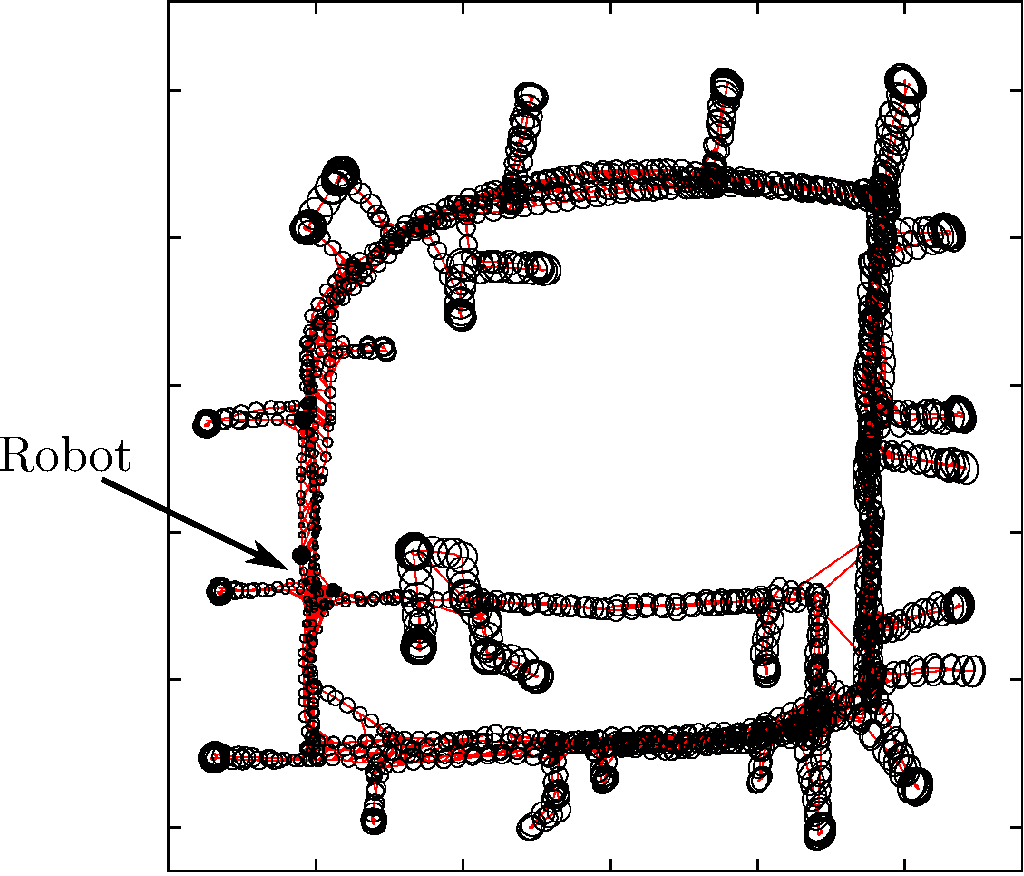
\includegraphics[width=0.2\textwidth]{pose_graph_relative_uncertainty.pdf}
    \end{figure}
    
    \end{frame}
    
    \begin{frame}
    \frametitle{Pose-Graph Summary}
    \note{Information taken from https://youtu.be/uHbRKvD8TWg}
    
    \begin{itemize}
    \item The back-end of the SLAM problem can be solved by applying Gauss-Newton
    \item The matrix $\linearSystemH$ is sparse
    \item That $\linearSystemH$ is sparse allows us to solve the linear system efficiently
    \end{itemize}
    
    \end{frame}
    
    \begin{frame}
    \frametitle{Graph-Based SLAM with Landmarks}
    \note{Information taken from https://youtu.be/mZBdPgBtrCM}
    
     \begin{figure}[!h]
     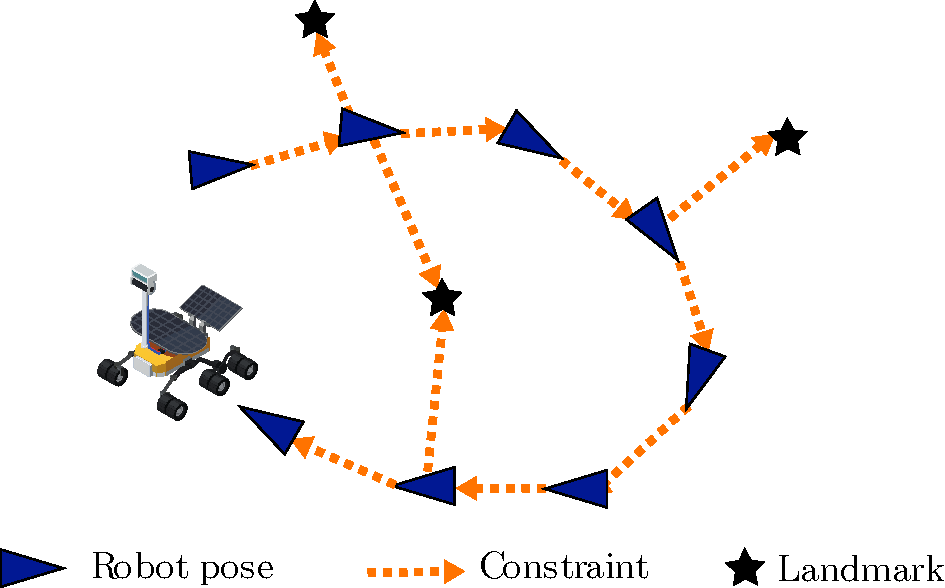
\includegraphics[width=0.6\textwidth]{images/pose_landmark_graph_example.pdf}
     \end{figure}
    
    \end{frame}
    
    \begin{frame}
     \frametitle{Landmark observations}
     \note{Information taken from https://youtu.be/mZBdPgBtrCM}
    
     \begin{tikzpicture}[remember picture,overlay]
     \node[xshift=-2.5cm,yshift=2cm] at (current page.east) { 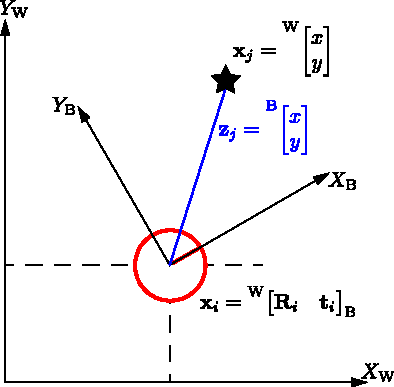
\includegraphics[height=0.5\textheight]{./images/landmark_observation_x_y_sensor.pdf}};
     \end{tikzpicture}
    \vspace{4em}
    \begin{itemize}
    \item Expected observation for an (x-y sensor\footnote{x-y sensor is a sensor whose measurements have the form (x,y), a point in the scene. In a 2D world.})
    \begin{figure}[!h]
    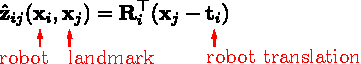
\includegraphics[width=0.6\textwidth]{images/pose_landmark_graph_expected_observation.pdf}
    \end{figure}
    \item Error function
    \begin{align*}
    \error_{ij}(\stateBold_{i}, \stateBold_{j}) &= \hat{\observationBold}_{ij} - \observationBold_{ij}\\
    &= \rotation_{i}^{\top}(\stateBold_{j}-\translation_{i}) - \observationBold_{ij}
     \end{align*}
     \end{itemize}
    
    \end{frame}
    
    \begin{frame}
     \frametitle{Bearing only observations (angle observations)}
     \note{Information taken from https://youtu.be/mZBdPgBtrCM}
    
     \begin{tikzpicture}[remember picture,overlay]
     \node[xshift=-2.5cm,yshift=2cm] at (current page.east) { 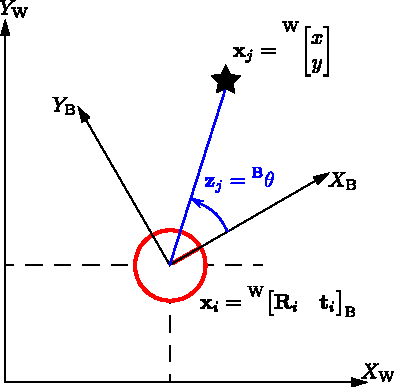
\includegraphics[height=0.5\textheight]{./images/landmark_observation_bearing_only_sensor.pdf}};
     \end{tikzpicture}
    
    
     \begin{itemize}
     \item A landmark is a 2D point
     \item The robot observes the angle towards the landmark
     \item Observation function
     \begin{figure}[!h]
     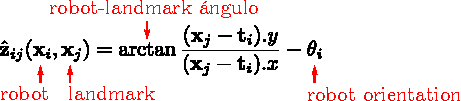
\includegraphics[width=0.6\textwidth]{images/pose_landmark_graph_bearing_observation.pdf}
     \end{figure}
     \item Error function
     \begin{equation*}
     \error _{ij}(\stateBold _{i},\stateBold _{j}) = \arctan{\dfrac{(\stateBold _{j}-\translation _{i}).y}{(\stateBold _{j}-\translation _{i}).x}} - \theta _{i} - \observationBold _{j}
     \end{equation*}
     \end{itemize}
    
    
\end{frame}

\begin{frame}
    \frametitle{Rank of matrix H}
    \note{Information taken from https://youtu.be/mZBdPgBtrCM}
    
    \begin{itemize}
    \item What is the rank of the matrix $\linearSystemH_{ij}$ for a 2D pose-landmark constraint?
    \begin{itemize}
    \item The rank of $\linearSystemH_{ij}$ is determined by the rank of the Jacobian $\jacobian_{ij}$ which is at most a $2 \times 5$ matrix (2 because the measurement gives 2D information and 5 for $\begin{bmatrix} x & y & \theta & l_{x} & l_{y} \end{bmatrix}$)
    \item $\linearSystemH_{ij}$ cannot have more than rank 2
    
    $rank(\linearSystemH_{ij}) = rank(\jacobian_{ij}^{\top} \informationMatrix_{ij} \jacobian_{ij}) = rank(\jacobian_{ij}) \quad \text{See: The Matrix Cookcook sec. 9.6.9}$
    \end{itemize}
    
    \item What is the rank of the matrix $\linearSystemH_{ij}$ for a pose-landmark bearing-only constraint?
    \begin{itemize}
    \item The rank of $\linearSystemH_{ij}$ is determined by the rank of the Jacobian $\jacobian_{ij}$ which is at most a $1 \times 5$ matrix. 1 because the measurement gives 1D information and 5 for $\begin{bmatrix} x & y & \theta & l_{x} & l_{y} \end{bmatrix}$
    \item $\linearSystemH_{ij}$ has rank 1
    \end{itemize}
    
    \end{itemize}
    \end{frame}
    
    \begin{frame}
    \frametitle{Where is the robot?}
    \note{Information taken from https://youtu.be/mZBdPgBtrCM}
    \begin{itemize}
    \item The robot observes a landmark $(x,y)$
    \item Where can the robot be relative to the landmark?
    \end{itemize}
    
    \only<1>{
    \begin{center}
    
\includegraphics[width=0.3\textwidth]{images/robot_pose_landmark_with_xy_sensor1.pdf}
    \end{center}
    }
    
    \only<2>{
    \begin{center}
    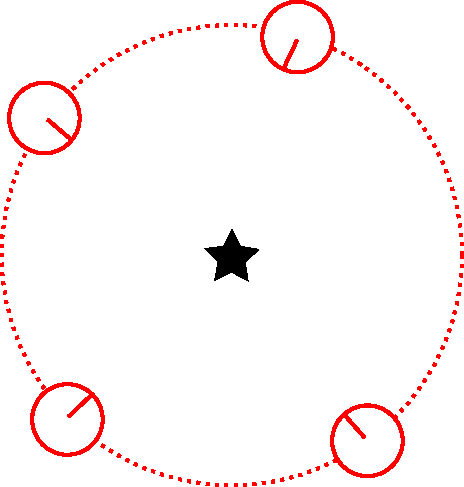
\includegraphics[width=0.3\textwidth]{images/robot_pose_landmark_with_xy_sensor2.pdf}
    \end{center}
    The robot can be anywhere on the circle.\\
    It is a 1D solution space (restricted by the robot's distance and orientation).
    }
    \end{frame}
    
    \begin{frame}
    \frametitle{Where is the robot?}
    \note{Information taken from https://youtu.be/mZBdPgBtrCM}
    \begin{itemize}
    \item The robot observes a landmark (bearing-only)
    \item Where can the robot be relative to the landmark?
    \end{itemize}
    
    \only<1>{
    \begin{center}
    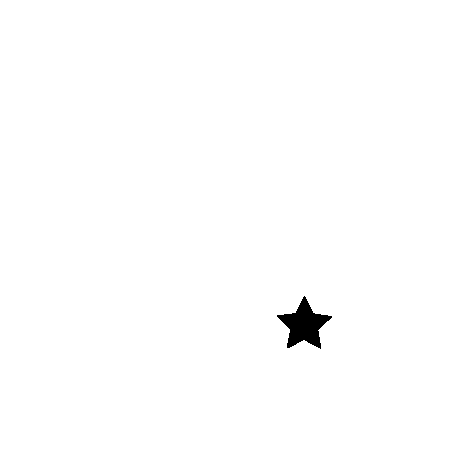
\includegraphics[width=0.3\textwidth]{images/robot_pose_landmark_with_bearing_sensor1.pdf}
    \end{center}
    }
    
    \only<2>{
    \begin{center}
    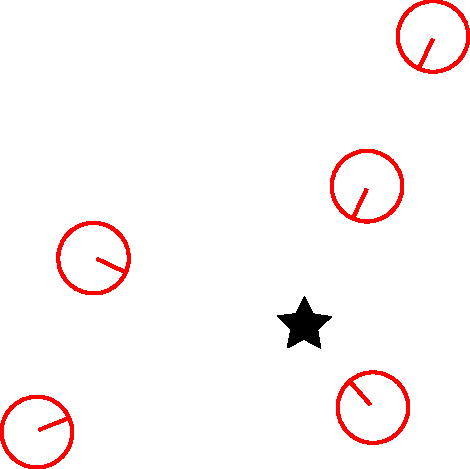
\includegraphics[width=0.3\textwidth]{images/robot_pose_landmark_with_bearing_sensor2.pdf}
    \end{center}
    The robot can be anywhere in the xy plane. It will always be pointing toward the landmark.
    It is a 2D solution space (restricted by the robot's orientation).
    }
    \end{frame}
    
    \begin{frame}
    \frametitle{Range}
    \note{Information taken from https://youtu.be/mZBdPgBtrCM}
    \begin{itemize}
    \item In SLAM with landmarks, the system can be indeterminate
    \item The rank of $\linearSystemH$ is {\bf less than or equal} to the sum of the ranks of all observations
    \item To determine a {\bf unique solution}, the system must have {\bf full rank}
    \end{itemize}
    
    \only<2-> {
    Questions:
    }
    
    \begin{itemize}
    \item<2-> How many landmark observations $(x,y)$ are needed to solve a robot's pose?
    \begin{itemize}
    \item<3-> At least 2 observations are required
    \end{itemize}
    \item<4-> How many bearing-only observations are needed to resolve a robot's pose?
    \begin{itemize}
    \item<5-> At least 3 observations are required
    \end{itemize}
    \end{itemize}
    \end{frame}
    
    \begin{frame}
    \frametitle{Indeterminate System}
    \note{Information taken from https://youtu.be/mZBdPgBtrCM}
    \begin{itemize}
    \item There is no guarantee that a system has full range
    \begin{itemize}
    \item Landmarks can only be observed once
    \item The robot may not have odometry information. \note{Odometry in general provides information about the entire pose.}
    \end{itemize}
    \item We can deal with these problems by using a \emph{damping factor} for $\linearSystemH$
    \item Instead of solving $\linearSystemH \vec{\Delta} \stateBold = - \linearSystemb$, we solve
    $(\linearSystemH + \lambda \vec{I}) \vec{\Delta} \stateBold = - \linearSystemb$
     \end{itemize}
\end{frame}

\begin{frame}
    \frametitle{Levenberg–Marquardt}
    \note{Información extraída de https://youtu.be/mZBdPgBtrCM}
    
    \footnotesize
    
    \begin{itemize}
        \item The damping factor $\lambda \vec{I}$ makes the system positive definite.
        \item It is a weighted sum of the Gauss-Newton method and the gradient descent method. \note{When lambda increases, H becomes negligible and Levenberg–Marquardt behaves like the gradient method. This is because the vector b has information from the Jacobian, and it could be solved to give the gradient descent equation. On the other hand, when lambda is very small, Levenberg–Marquardt behaves like the Gauss-Newton method. Intuitively, Levenberg–Marquardt behaves like Gauss–Newton when it is close to the minimum (lambda decreases) and like gradient descent when it is far from the minimum (lambda increases).}
        \item The damping factor regulates convergence using backup/restore actions.
        \end{itemize}
        
    \begin{algorithmic}[1]
        \Procedure{Levenberg–Marquardt}{$\stateBold$} \Comment{$\stateBold$: initial seed}
        \While (!converged)
        \State $\lambda =  \lambda_{\textrm{init}}$
        \State $<\linearSystemH, \linearSystemb> = buildLinearSystem(\stateBold)$
        \State $E = error(\stateBold)$
        \State $\stateBold_{\textrm{old}} = \stateBold$
        \State $\vec{\Delta}\stateBold = solveSparse((\linearSystemH + \lambda \vec{I}) \vec{\Delta} \stateBold = - \linearSystemb)$
        \State $\stateBold \mathrel{+}= \vec{\Delta}\stateBold$
        \If{$E < error(\stateBold)$}
        \State $\stateBold = \stateBold_{\textrm{old}}$
        \State $\lambda \mathrel{*}= 2$
        \Else
        \State $\lambda \mathrel{/}= 2$
        \EndIf
        \EndWhile
        \EndProcedure
    \end{algorithmic}

\end{frame}
